\documentclass[12pt, a4paper, oneside]{memoir}
\usepackage{hyperref}
\usepackage{graphicx}
\usepackage{epsfig}
\usepackage{amsmath}
\usepackage{amssymb}
\usepackage{amsthm}
\usepackage{booktabs}
\usepackage{stmaryrd}
\usepackage{url}
\usepackage{float}
\usepackage{longtable}
\usepackage[figuresright]{rotating}
\usepackage[utf8]{inputenc}
\usepackage[T1]{fontenc}
\usepackage{lmodern}
\usepackage[polish]{babel}
\usepackage{indentfirst}
\usepackage{eso-pic}
\usepackage[ruled,vlined]{algorithm2e}
\usepackage{algorithmicx}
\usepackage{listings}
\usepackage{listingsutf8}
\usepackage{citeref}
\usepackage{color}
\usepackage{memhfixc}
\usepackage{pdfpages}
\usepackage{copyrightbox}
\usepackage{attachfile2}
\usepackage{siunitx}
\usepackage{currency}

\renewcommand\familydefault{\sfdefault}
\renewcommand{\bibitempages}[1]{\newblock {\scriptsize [\mbox{str.\ }#1]}}
\renewcommand{\emph}[1]{\textit{#1}}
\renewcommand\sf{\sffamily}

\definecolor{greenyellow}   {cmyk}{0.15,    0, 0.69,    0}
\definecolor{yellow}        {cmyk}{   0,    0,    1,    0}
\definecolor{goldenrod}     {cmyk}{   0, 0.10, 0.84,    0}
\definecolor{dandelion}     {cmyk}{   0, 0.29, 0.84,    0}
\definecolor{apricot}       {cmyk}{   0, 0.32, 0.52,    0}
\definecolor{peach}         {cmyk}{   0, 0.50, 0.70,    0}
\definecolor{melon}         {cmyk}{   0, 0.46, 0.50,    0}
\definecolor{yelloworange}  {cmyk}{   0, 0.42,    1,    0}
\definecolor{orange}        {cmyk}{   0, 0.61, 0.87,    0}
\definecolor{burntorange}   {cmyk}{   0, 0.51,    1,    0}
\definecolor{bittersweet}   {cmyk}{   0, 0.75,    1, 0.24}
\definecolor{redorange}     {cmyk}{   0, 0.77, 0.87,    0}
\definecolor{mahogany}      {cmyk}{   0, 0.85, 0.87, 0.35}
\definecolor{maroon}        {cmyk}{   0, 0.87, 0.68, 0.32}
\definecolor{brickred}      {cmyk}{   0, 0.89, 0.94, 0.28}
\definecolor{red}           {cmyk}{   0,    1,    1,    0}
\definecolor{orangered}     {cmyk}{   0,    1, 0.50,    0}
\definecolor{rubinered}     {cmyk}{   0,    1, 0.13,    0}
\definecolor{wildstrawberry}{cmyk}{   0, 0.96, 0.39,    0}
\definecolor{salmon}        {cmyk}{   0, 0.53, 0.38,    0}
\definecolor{carnationpink} {cmyk}{   0, 0.63,    0,    0}
\definecolor{magenta}       {cmyk}{   0,    1,    0,    0}
\definecolor{violetred}     {cmyk}{   0, 0.81,    0,    0}
\definecolor{rhodamine}     {cmyk}{   0, 0.82,    0,    0}
\definecolor{mulberry}      {cmyk}{0.34, 0.90,    0, 0.02}
\definecolor{redviolet}     {cmyk}{0.07, 0.90,    0, 0.34}
\definecolor{fuchsia}       {cmyk}{0.47, 0.91,    0, 0.08}
\definecolor{lavender}      {cmyk}{   0, 0.48,    0,    0}
\definecolor{thistle}       {cmyk}{0.12, 0.59,    0,    0}
\definecolor{orchid}        {cmyk}{0.32, 0.64,    0,    0}
\definecolor{darkorchid}    {cmyk}{0.40, 0.80, 0.20,    0}
\definecolor{purple}        {cmyk}{0.45, 0.86,    0,    0}
\definecolor{plum}          {cmyk}{0.50,    1,    0,    0}
\definecolor{violet}        {cmyk}{0.79, 0.88,    0,    0}
\definecolor{royalpurple}   {cmyk}{0.75, 0.90,    0,    0}
\definecolor{blueviolet}    {cmyk}{0.86, 0.91,    0, 0.04}
\definecolor{periwinkle}    {cmyk}{0.57, 0.55,    0,    0}
\definecolor{cadetblue}     {cmyk}{0.62, 0.57, 0.23,    0}
\definecolor{cornflowerblue}{cmyk}{0.65, 0.13,    0,    0}
\definecolor{midnightblue}  {cmyk}{0.98, 0.13,    0, 0.43}
\definecolor{navyblue}      {cmyk}{0.94, 0.54,    0,    0}
\definecolor{royalblue}     {cmyk}{   1, 0.50,    0,    0}
\definecolor{blue}          {cmyk}{   1,    1,    0,    0}
\definecolor{cerulean}      {cmyk}{0.94, 0.11,    0,    0}
\definecolor{cyan}          {cmyk}{   1,    0,    0,    0}
\definecolor{processblue}   {cmyk}{0.96,    0,    0,    0}
\definecolor{skyblue}       {cmyk}{0.62,    0, 0.12,    0}
\definecolor{turquoise}     {cmyk}{0.85,    0, 0.20,    0}
\definecolor{tealblue}      {cmyk}{0.86,    0, 0.34, 0.02}
\definecolor{aquamarine}    {cmyk}{0.82,    0, 0.30,    0}
\definecolor{bluegreen}     {cmyk}{0.85,    0, 0.33,    0}
\definecolor{emerald}       {cmyk}{   1,    0, 0.50,    0}
\definecolor{junglegreen}   {cmyk}{0.99,    0, 0.52,    0}
\definecolor{seagreen}      {cmyk}{0.69,    0, 0.50,    0}
\definecolor{green}         {cmyk}{   1,    0,    1,    0}
\definecolor{forestgreen}   {cmyk}{0.91,    0, 0.88, 0.12}
\definecolor{pinegreen}     {cmyk}{0.92,    0, 0.59, 0.25}
\definecolor{limegreen}     {cmyk}{0.50,    0,    1,    0}
\definecolor{yellowgreen}   {cmyk}{0.44,    0, 0.74,    0}
\definecolor{springgreen}   {cmyk}{0.26,    0, 0.76,    0}
\definecolor{olivegreen}    {cmyk}{0.64,    0, 0.95, 0.40}
\definecolor{rawsienna}     {cmyk}{   0, 0.72,    1, 0.45}
\definecolor{sepia}         {cmyk}{   0, 0.83,    1, 0.70}
\definecolor{brown}         {cmyk}{   0, 0.81,    1, 0.60}
\definecolor{tan}           {cmyk}{0.14, 0.42, 0.56,    0}
\definecolor{gray}          {cmyk}{   0,    0,    0, 0.50}
\definecolor{black}         {cmyk}{   0,    0,    0,    1}
\definecolor{white}         {cmyk}{   0,    0,    0,    0}
\definecolor{mygray}        {cmyk}{0.03, 0.03, 0.03, 0.03}

\bibliographystyle{plain}

\lstset{
	basicstyle=\footnotesize\ttfamily,
	keywordstyle=\color{blue},
	stringstyle=\color{violetred},
	commentstyle=\color{green}, 
	frame=single,
	frameround=tttt,
	framesep=5pt,
    inputencoding=utf8/cp1250,
    breaklines=true,
    postbreak=\mbox{\textcolor{red}{$\hookrightarrow$}\space},
}

\ifpdf
    \hypersetup{
        plainpages=false,
        bookmarksnumbered,
        colorlinks=true,
        linkcolor=black,
        citecolor=black,
        filecolor=black,
        urlcolor=black,
        unicode
    }
    \pdfimageresolution=600
    \pdfcompresslevel=9
    \usepackage{thumbpdf}
\fi

\attachfilesetup{
    color=black
}

\newcounter{ax}
\newlistof{listofappendices}{loa}{Spis załączników}
\DeclareDocumentCommand{\ax}{ m m o }{%
    \refstepcounter{ax}%
    \textattachfile[#3]{#2}{#1~[F\theax]}%
    \addcontentsline{loa}{ax}{\protect\numberline{F\theax}#1}%
}
\makeatletter
\let\l@ax\l@figure
\makeatother

\sisetup{locale=PL}
\DefineCurrency{PLN}{
    iso=PLN,
    kind=symbol,
    name={złoty},
    plural={złotych},
    symbol={zł},
}

\settypeblocksize{23cm}{16cm}{*}

\setlrmargins{*}{2 cm}{*}
\setulmargins{*}{*}{1.3}

\setheadfoot{\onelineskip}{2\onelineskip}
\setheaderspaces{*}{2\onelineskip}{*}

\renewcommand\baselinestretch{1.3}

\checkandfixthelayout

\makechapterstyle{mychapterstyle}{%
    \renewcommand{\chapnamefont}{\LARGE\sffamily\bfseries}%
    \renewcommand{\chapnumfont}{\LARGE\sffamily\bfseries}%
    \renewcommand{\chaptitlefont}{\Huge\sffamily\bfseries}%
    \renewcommand{\printchaptertitle}[1]{%
        \chaptitlefont\hrule height 0.5 pt \vspace{1em}%
        {##1}\vspace{1em}\hrule height 0.5 pt%
    }%
    \renewcommand{\printchapternum}{%
        \chapnumfont\thechapter%
    }%
}

\chapterstyle{mychapterstyle}

\setsecheadstyle{\Large\sffamily\bfseries}
\setsubsecheadstyle{\large\sffamily\bfseries}
\setsubsubsecheadstyle{\normalfont\sffamily\bfseries}
\setparaheadstyle{\normalfont\sffamily}

\makeevenhead{headings}{\thepage}{}{\small\slshape\leftmark}
\makeoddhead{headings}{\small\slshape\rightmark}{}{\thepage}

\settocdepth{subsection}

\setsecnumdepth{subsection}
\maxsecnumdepth{subsection}
\settocdepth{subsection}
\maxtocdepth{subsection}

\setlength{\epigraphwidth}{0.57\textwidth}
\setlength{\epigraphrule}{0pt}
\setlength{\beforeepigraphskip}{1\baselineskip}
\setlength{\afterepigraphskip}{2\baselineskip}

\setlength{\parskip}{2mm}

\newcommand{\epitext}{\sffamily\itshape}
\newcommand{\epiauthor}{\sffamily\scshape ---~}
\newcommand{\epititle}{\sffamily\itshape}
\newcommand{\epidate}{\sffamily\scshape}
\newcommand{\episkip}{\medskip}

\newcommand{\myepigraph}[4]{%
	\epigraph{\epitext #1\episkip}{\epiauthor #2\\\epititle #3 \epidate(#4)}\noindent%
}

\renewcommand{\thefootnote}{\fnsymbol{footnote}}

\renewcommand{\today}{
    \ifcase \month%
        \or Styczeń\or Luty\or Marzec\or Kwiecień\or Maj \or Czerwiec\or Lipiec\or Sierpień\or Wrzesień\or Październik\or Listopad\or Grudzień%
    \fi~ \number \year%
}

\let\mainmatterorig\mainmatter
\renewcommand\mainmatter{%
    \edef\temppagenumber{\arabic{page}}%
	\mainmatterorig
	\setcounter{page}{\temppagenumber}%
}

\newcommand{\link}[1]{\href{https://#1}{\nolinkurl{#1}}}
\newcommand{\RNum}[1]{\uppercase\expandafter{\romannumeral #1\relax}}

\pagestyle{empty}
\begin{document}

\setcounter{figure}{0}
\setcounter{chapter}{1}
{\chapnamefont \thechapter. Informacje wstępne}

\section{Raspberry Pi}\label{sec:rpi}

Na~poniższym rysunku [\ref{fig:board}] płytki \emph{Raspberry Pi} kolorem zielonym zaznaczone~jest złącze \emph{GPIO},
wszystkie dalsze rysunki będą w~tej~samej orientacji -- z~tym~złączem po~górnej stronie rysunku.
Kolorem jasnoniebieskim zaznaczone są~złączki mocujące moduły podrzędne, można wykorzystać~je wraz~z~plastikowymi
śrubkami do~bezpieczniejszego przymocowania modułów.

Moduły mocuje~się wciskając znajdujące się po~ich dolnej stronie panel pasujący~do interfejsu \emph{GPIO} i~opcjonalnie
przykręcając złączki.
Moduły są zaprojektowane w~taki sposób, że~w~prawidłowej orientacji nie~wystają poza~granice płytki \emph{Raspberry Pi}.

\begin{figure}[H]
  \centering
  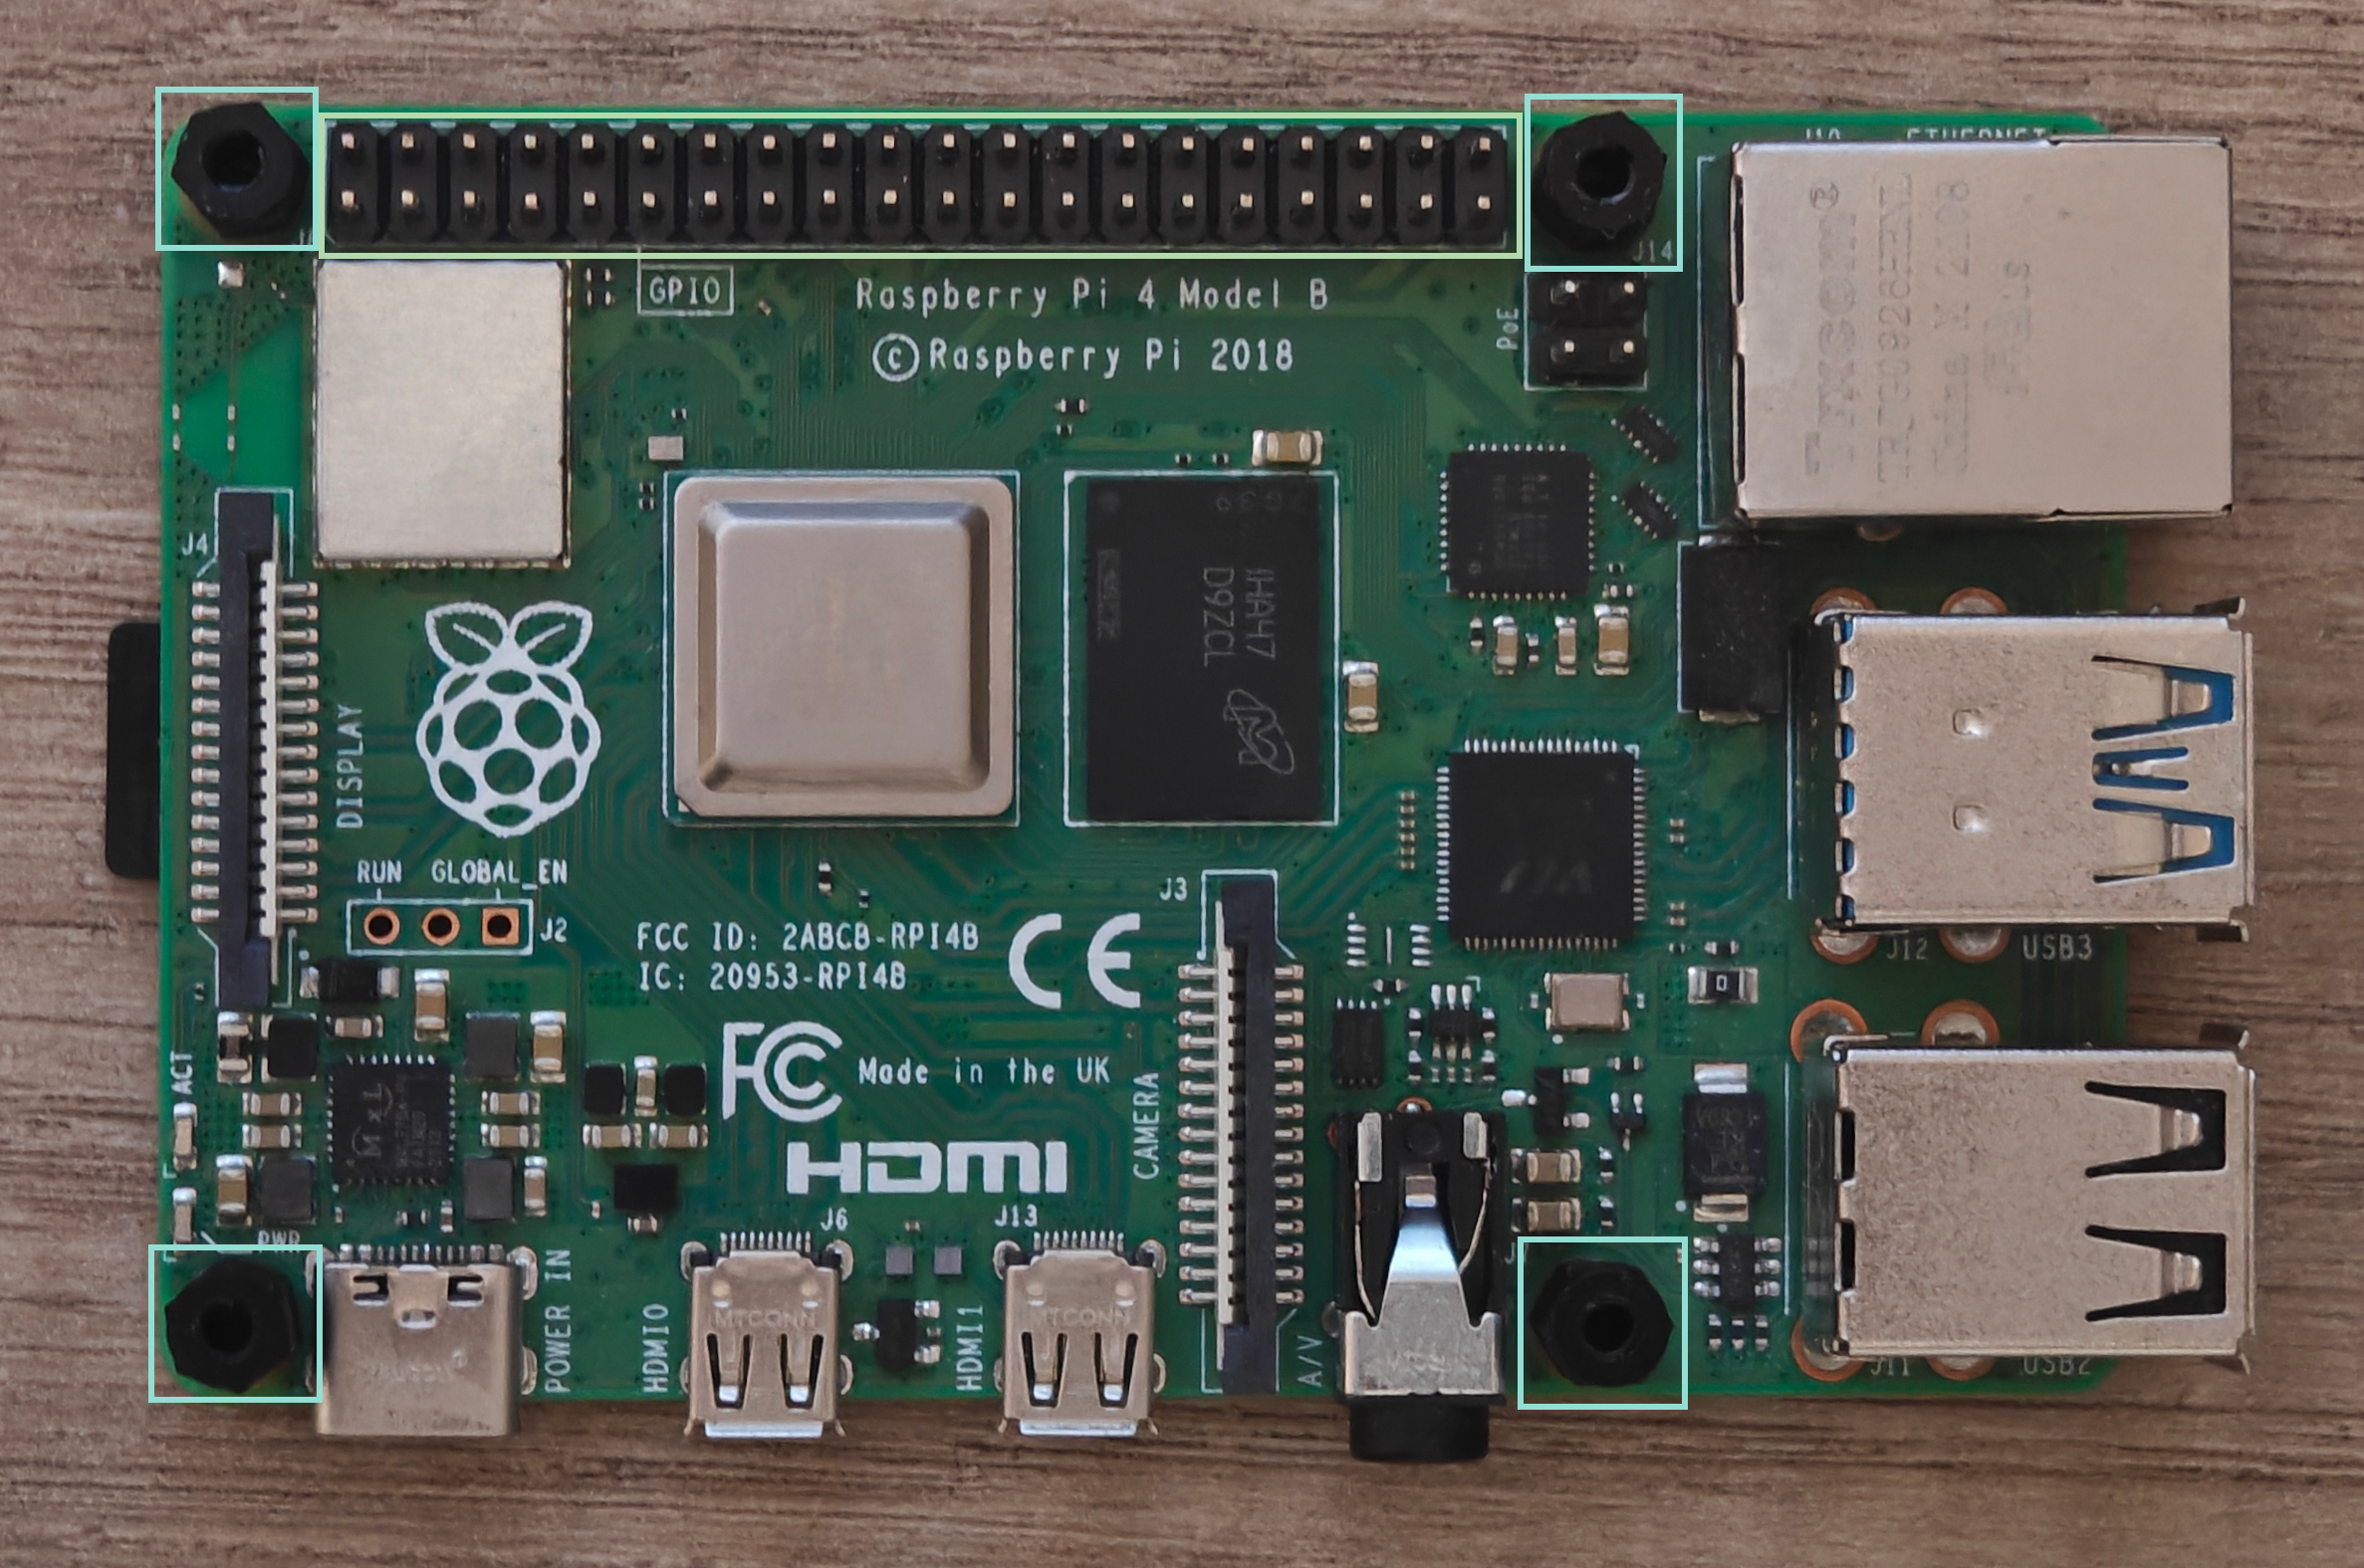
\includegraphics[width=0.8\linewidth]{media/board}\\
  \caption{Płytka \emph{Raspberry Pi}}
  \label{fig:board}
\end{figure}

\newpage
\section{Grove Base HAT}\label{sec:grove}

\emph{Grove Base HAT} jest~wykorzystany w~dwóch zadaniach.
\emph{Grove Base HAT} odwrócony tak, aby~widzieć jego~port \emph{GPIO} obok~portu \emph{GPIO} płytki
[\ref{fig:grovehatunbuilt}], ma~wcięcie (zaznaczone kolorem czerwonym) po~prawej stronie oraz~szczelinę (kolor żółty)
po~lewej dolnej stronie.
Montaż w~obu~przypadkach jest~identyczny, a~różni~się jedynie przymocowaniem rozszerzeń do~modułu Grove.

\begin{figure}[H]
  \centering
  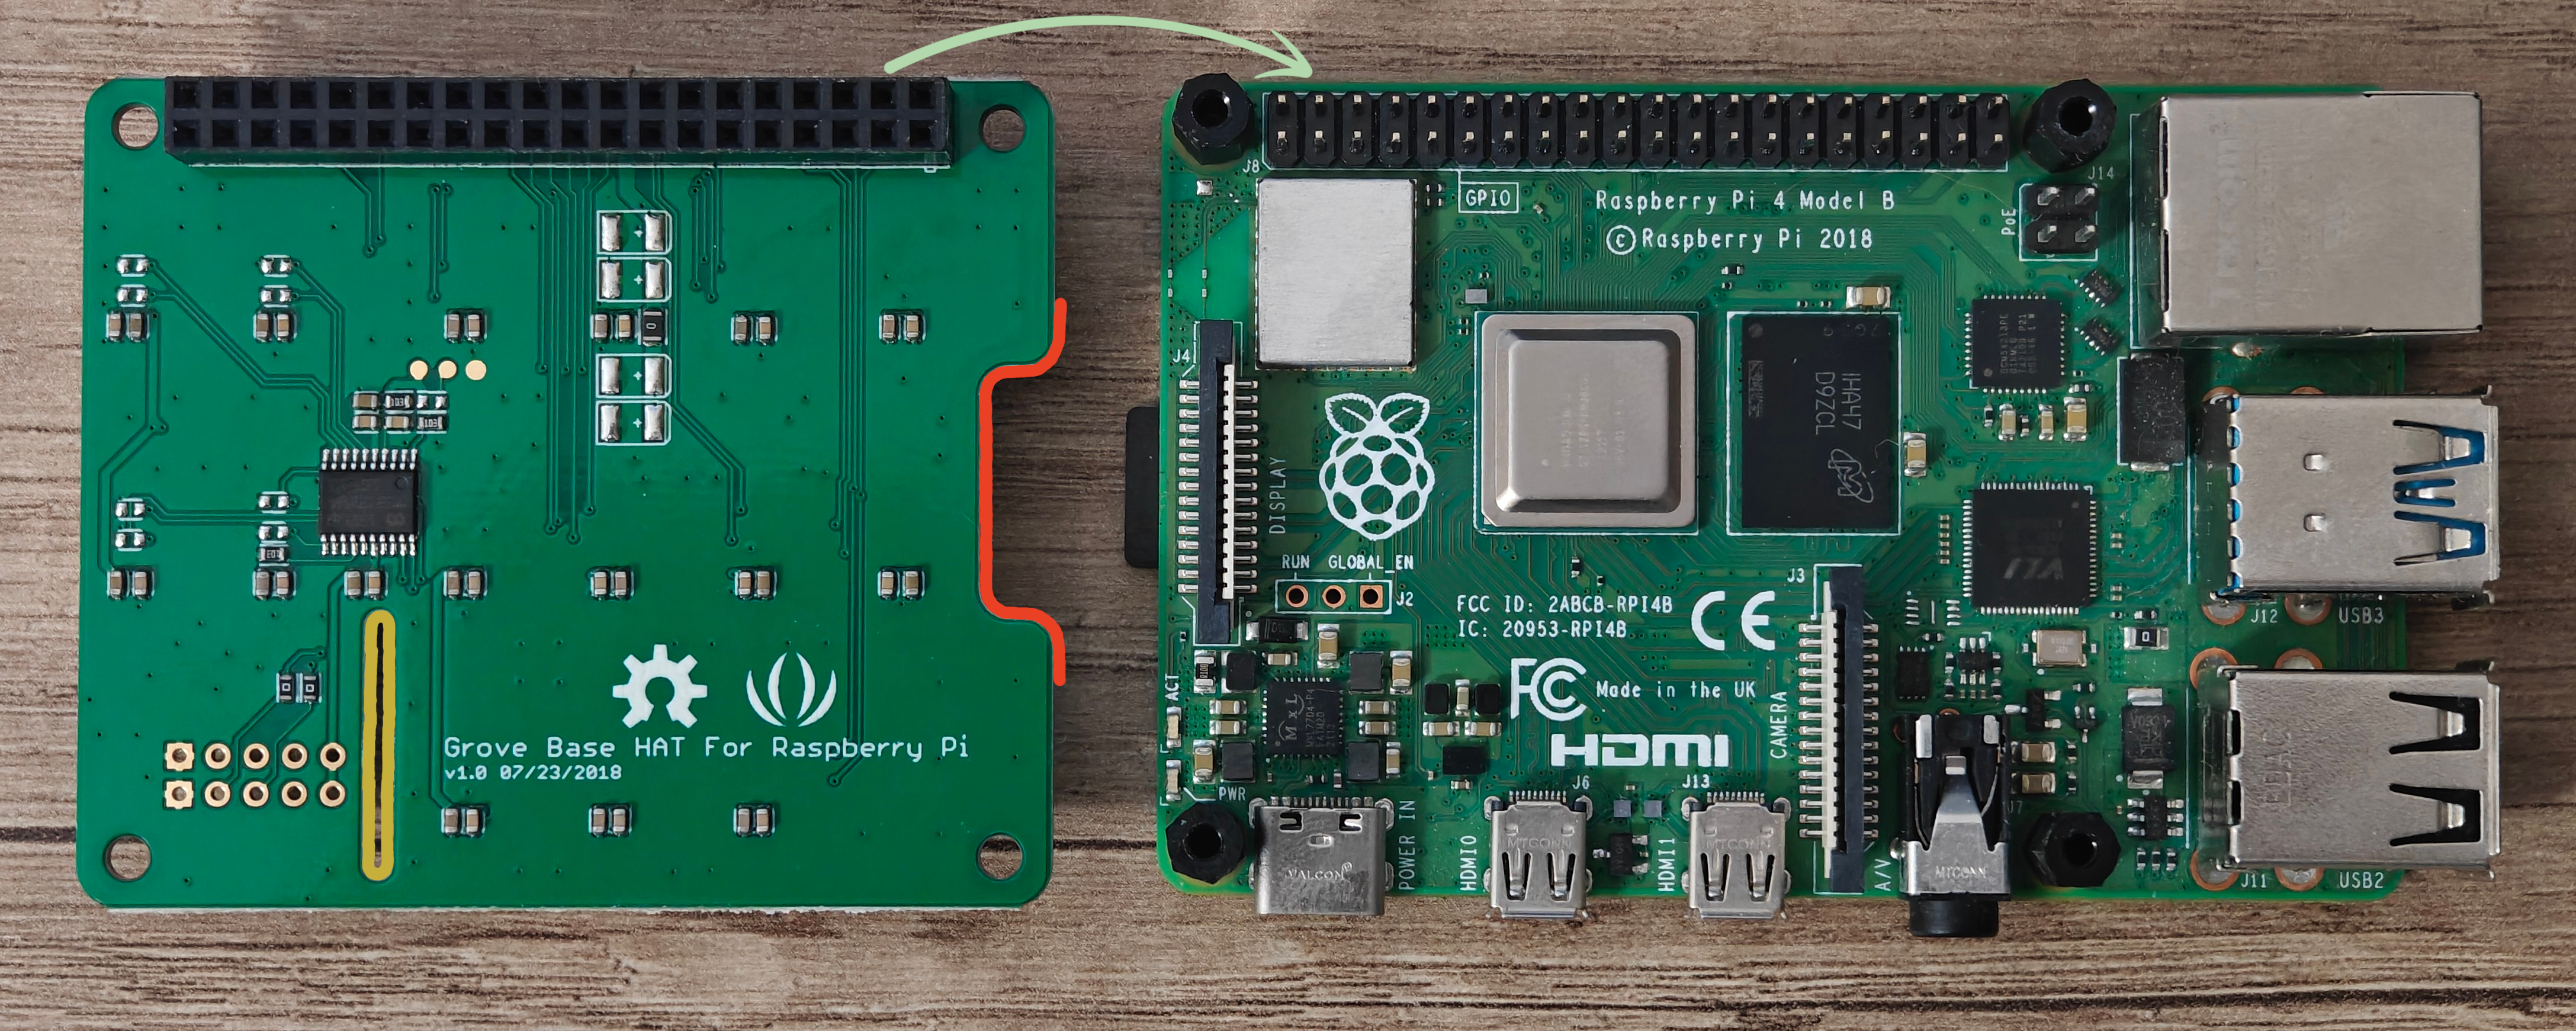
\includegraphics[width=\linewidth]{media/grove_hat_unbuilt}\\
  \caption{Moduł \emph{Grove Base HAT} obok płytki}
  \label{fig:grovehatunbuilt}
\end{figure}

Przymocowanie sprawi, że~to~wcięcie będzie po~stronie lewej, a~szczelina po~prawej, ale~nadal na~dole
[\ref{fig:grovehatbuilt}].

\begin{figure}[H]
  \centering
  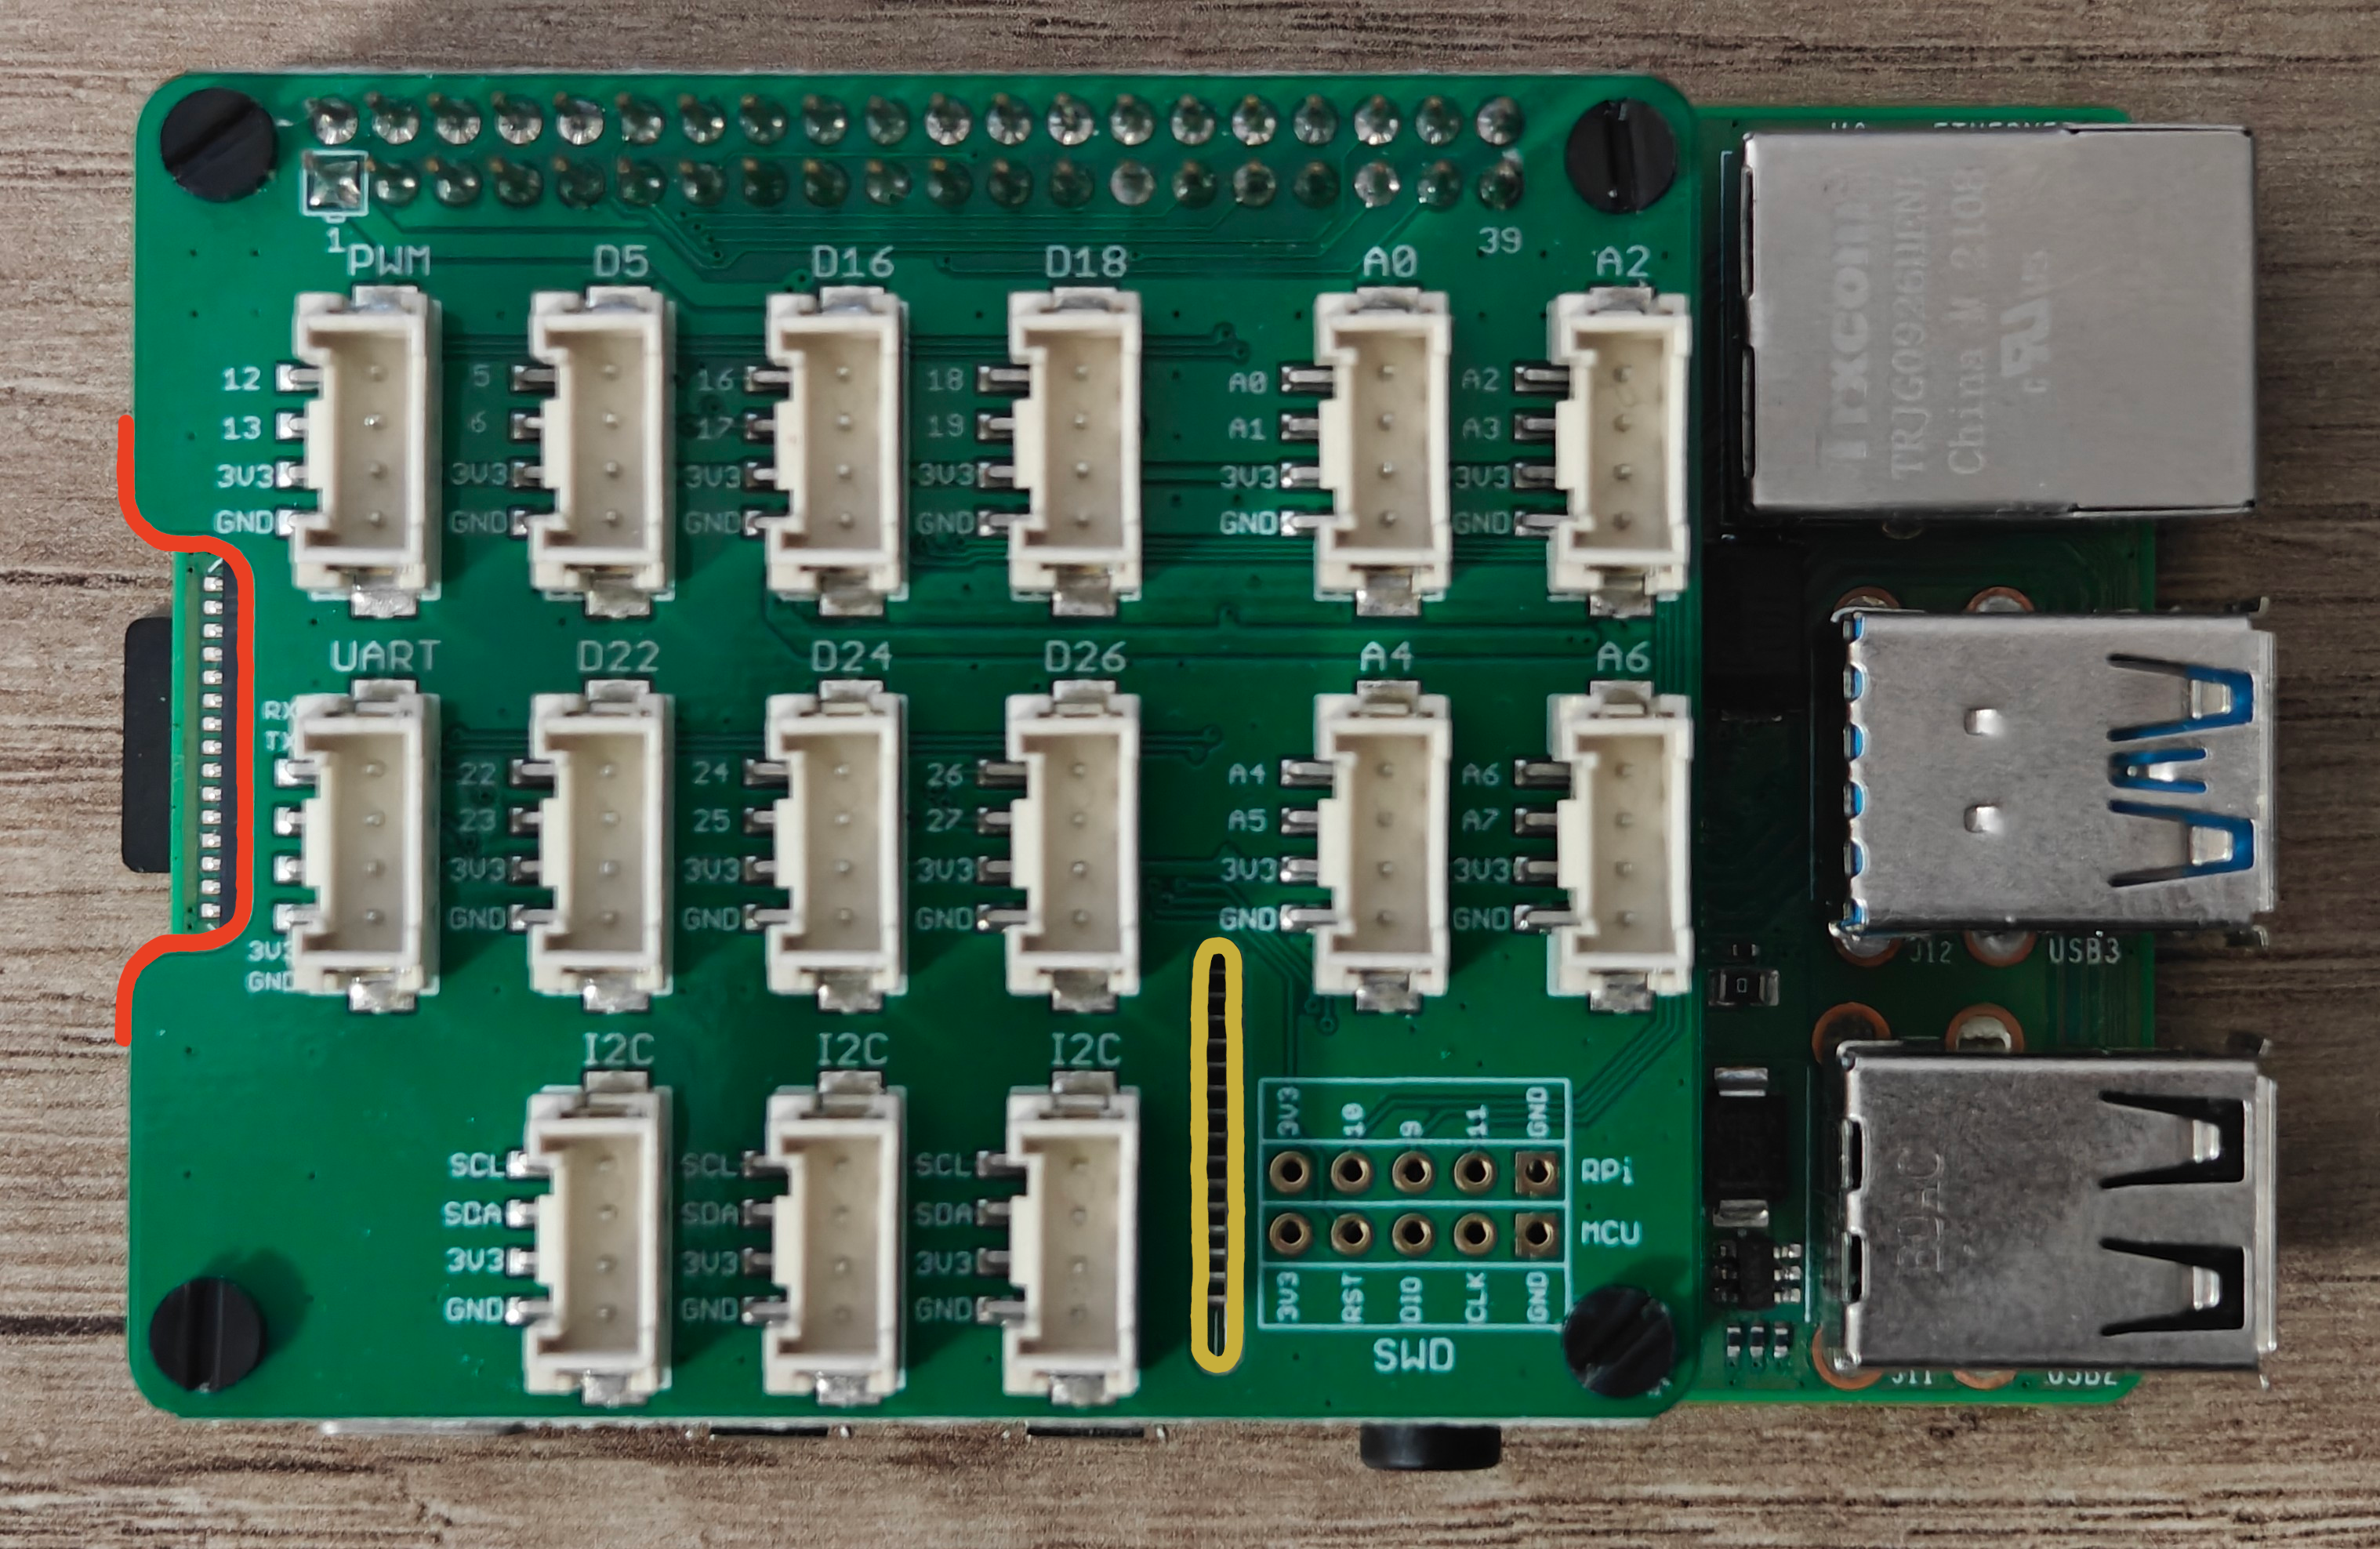
\includegraphics[width=0.6\linewidth]{media/grove_hat_built}\\
  \caption{Przymocowany moduł \emph{Grove Base HAT}}
  \label{fig:grovehatbuilt}
\end{figure}

\newpage
\setcounter{figure}{0}
\setcounter{chapter}{2}
{\chapnamefont \thechapter. Laboratorium I}

W~tym laboratorium wykorzystano moduł \emph{Sense HAT}\@.
Na rysunku [\ref{fig:sensehatunbuilt}] użyto te~same kolory pomocnicze, co~w~przypadku \emph{Grove Base HAT}\@.

\begin{figure}[H]
  \centering
  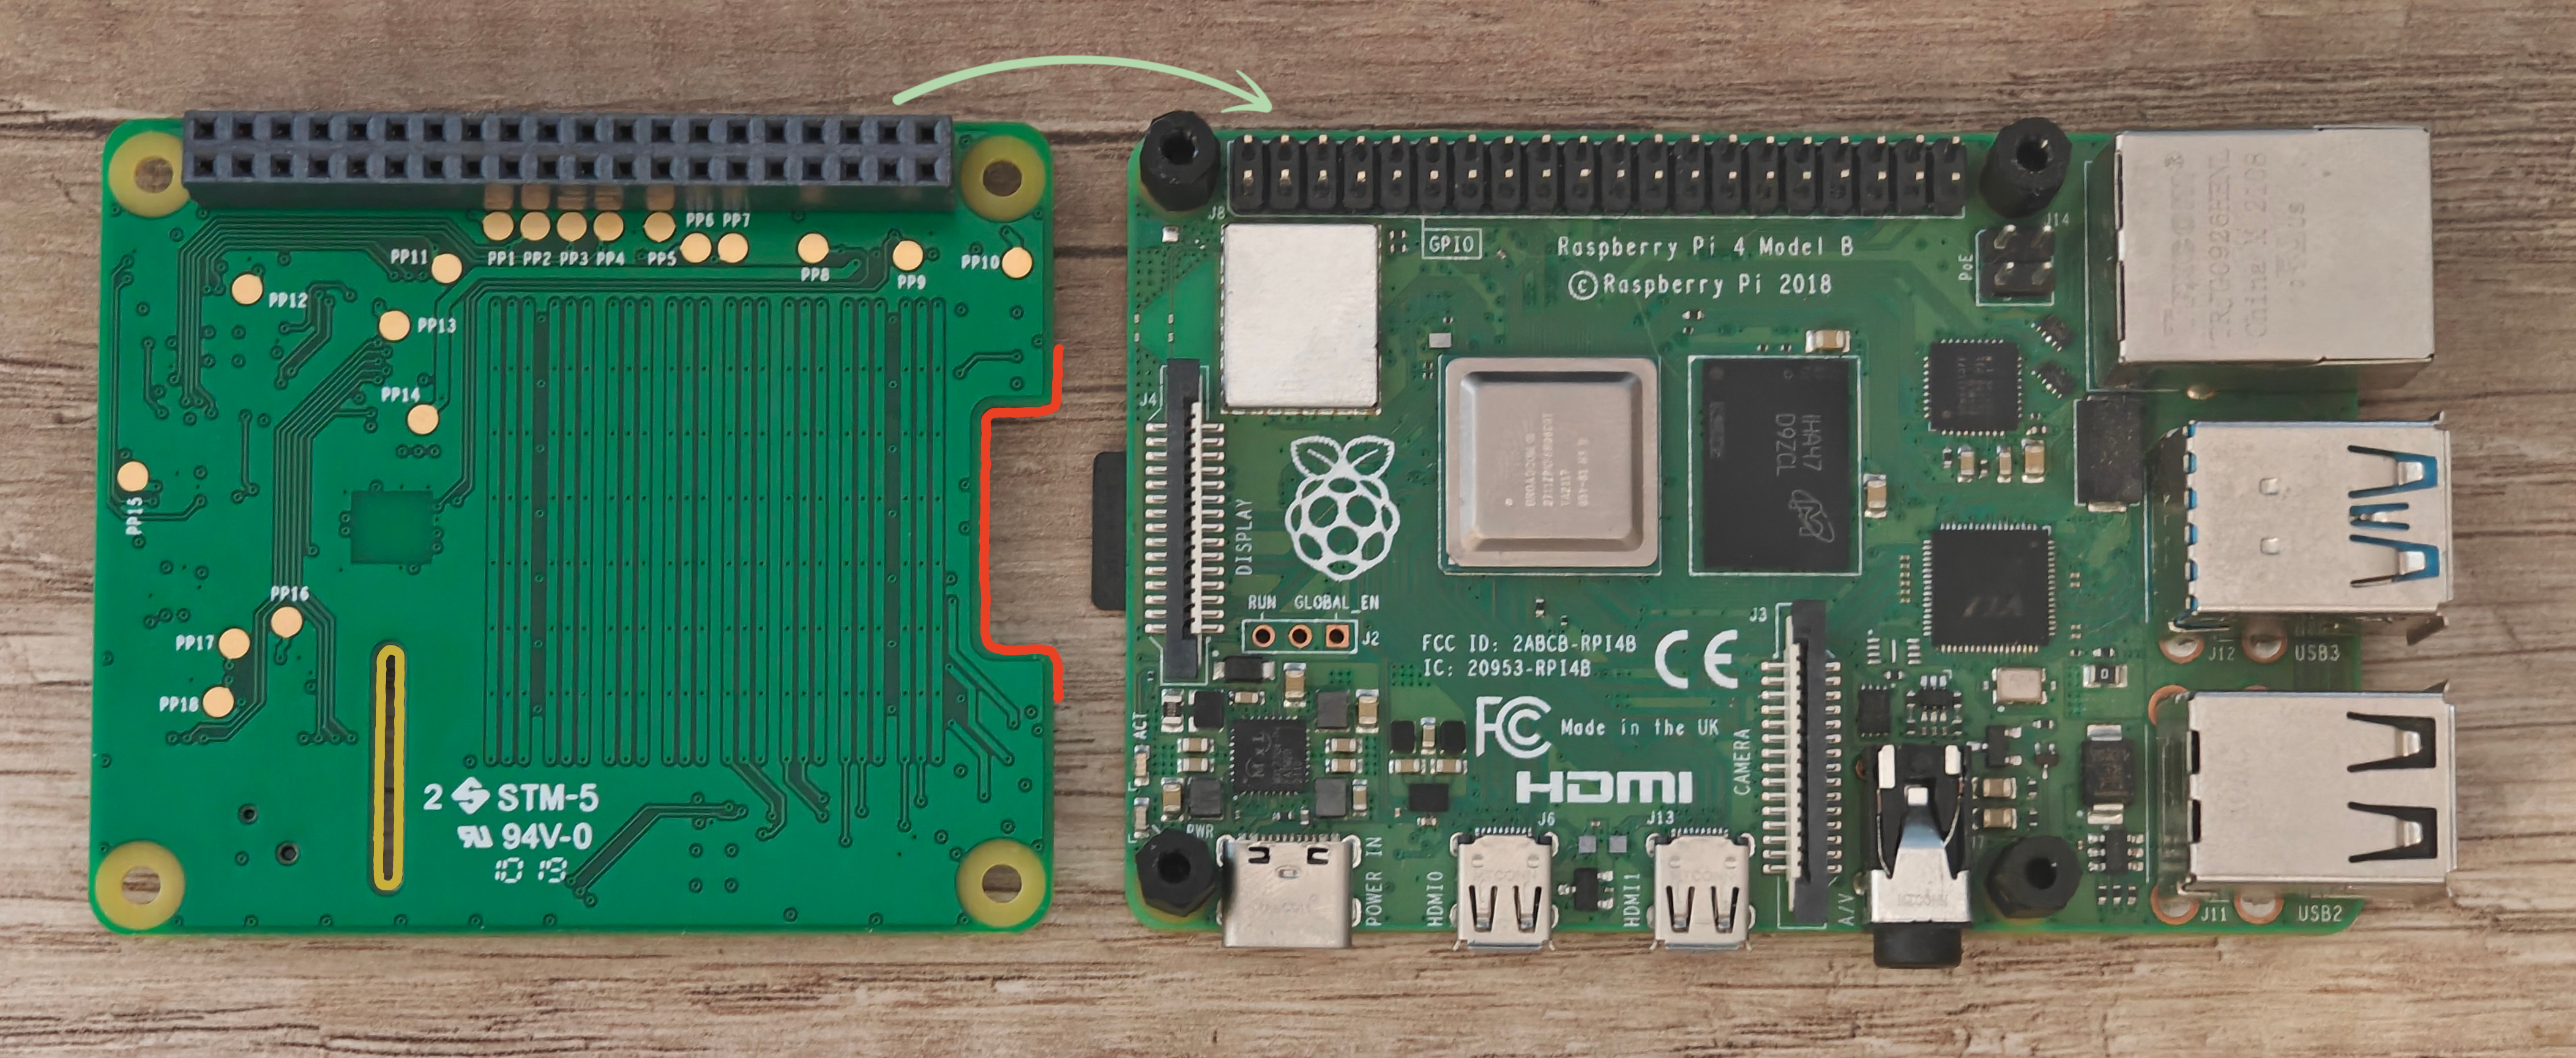
\includegraphics[width=\linewidth]{media/sense_hat_unbuilt}\\
  \caption{Moduł \emph{Sense HAT} obok płytki}
  \label{fig:sensehatunbuilt}
\end{figure}

Przymocowanie sprawi, że~to~wcięcie będzie po~stronie lewej, a~szczelina po~prawej, ale~nadal na~dole
[\ref{fig:sensehatbuilt}].

\begin{figure}[H]
  \centering
  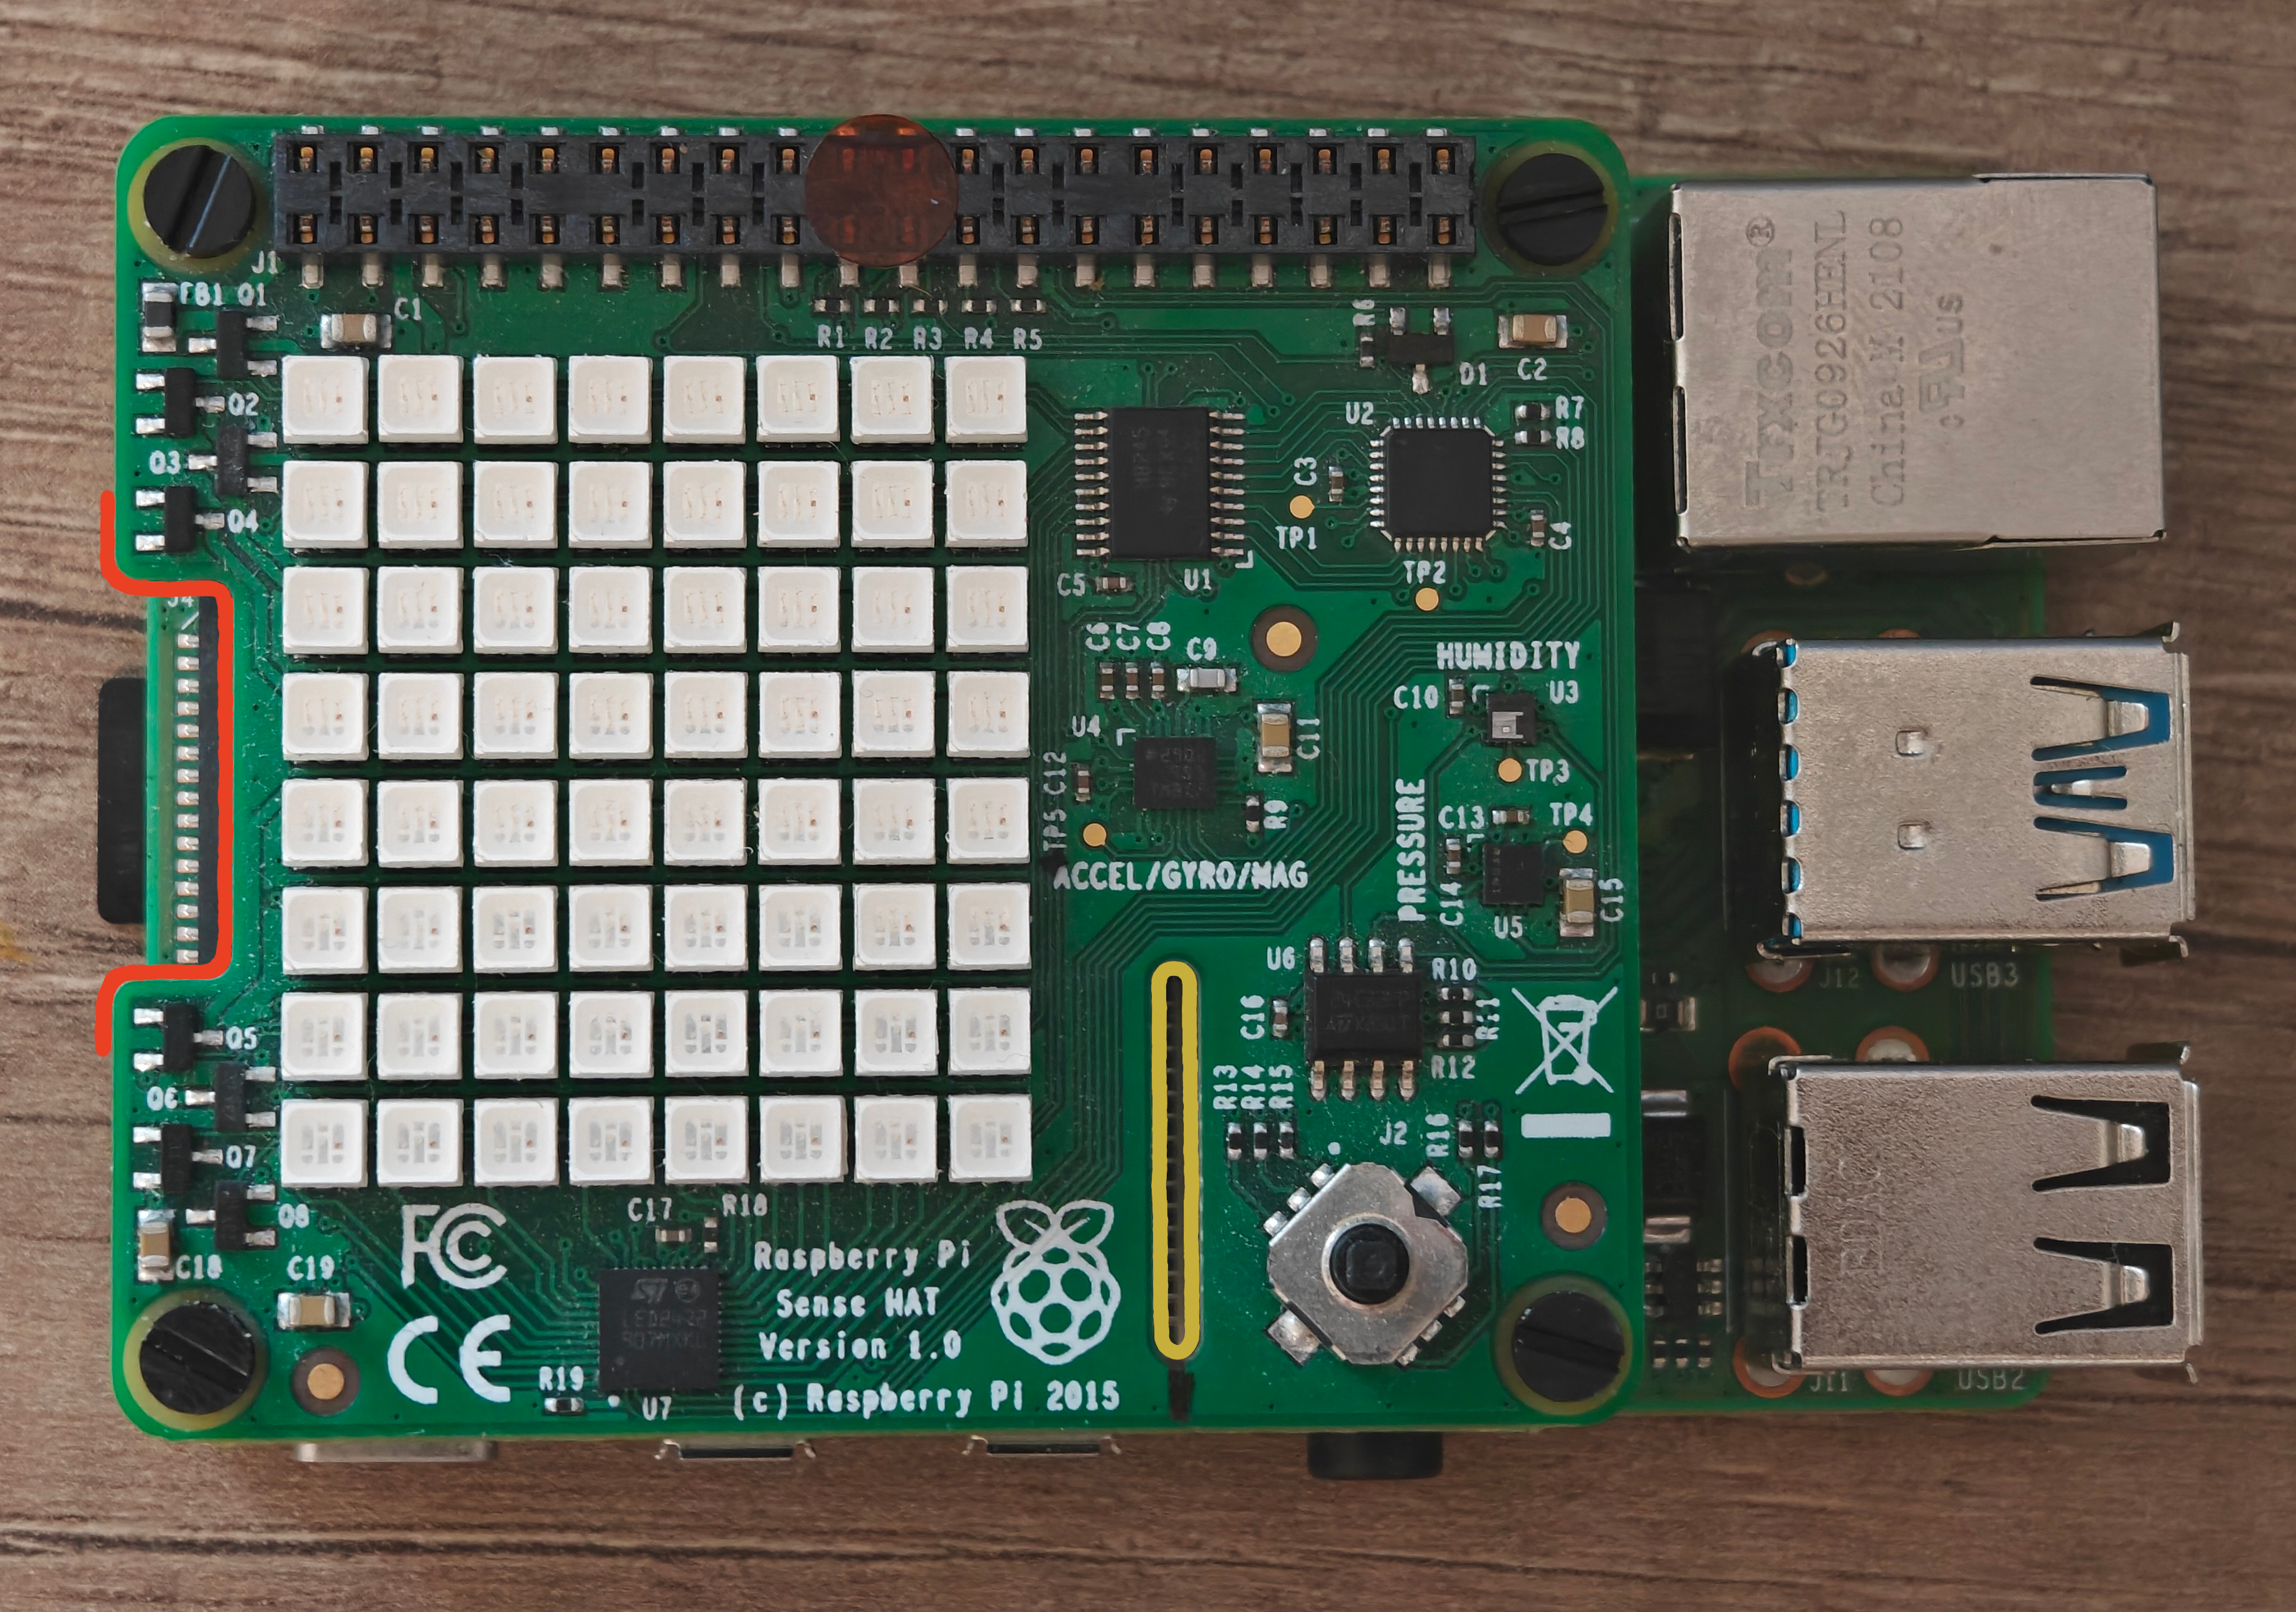
\includegraphics[width=0.6\linewidth]{media/sense_hat_built}\\
  \caption{Przymocowany moduł \emph{Sense HAT}}
  \label{fig:sensehatbuilt}
\end{figure}

\newpage
\setcounter{figure}{0}
\setcounter{chapter}{3}
{\chapnamefont \thechapter. Laboratorium II}

Laboratorium wykorzystuje \emph{Grove Base HAT}, podłącz najpierw ten~moduł.

Wyświetlacz LCD wykorzystuje port \textbf{\emph{I²C}}\@.
Laboratorium zawiera zadanie odczytania podłączonego numeru portu -- wykorzystaj losowy z portów \emph{I²C} (kolor
jasnozielony) [\ref{fig:grovelcd}].

\begin{figure}[H]
  \centering
  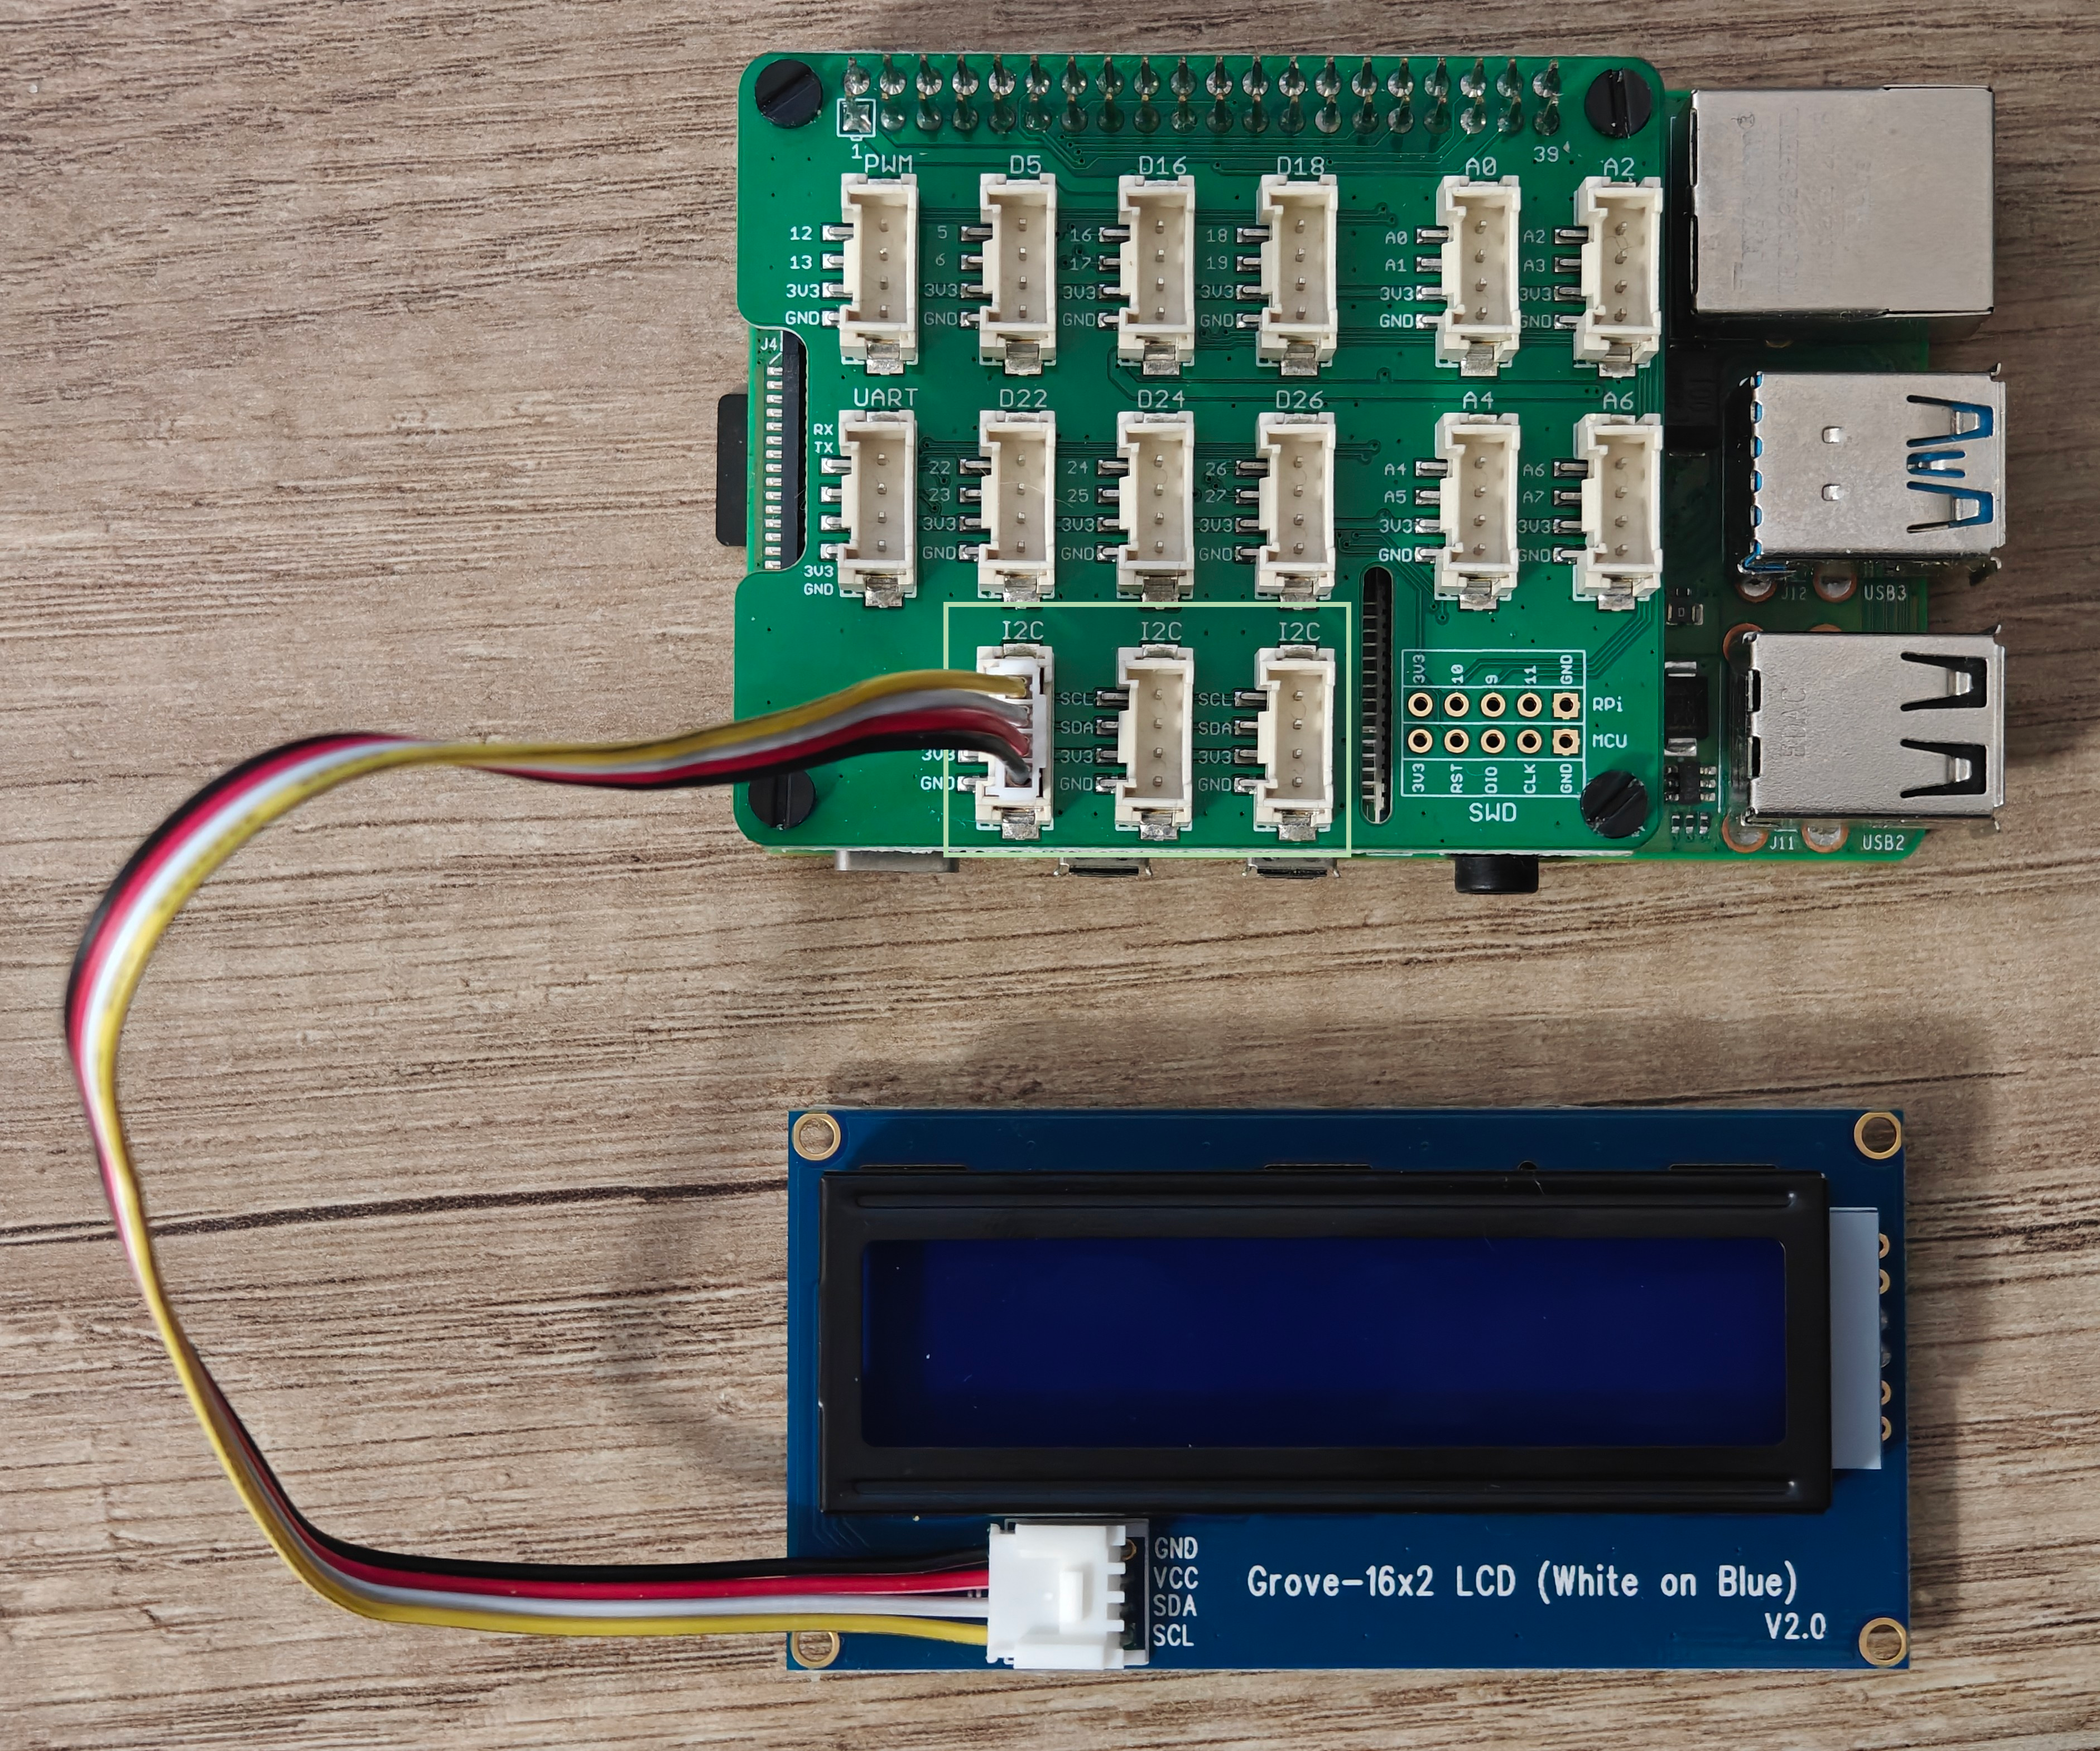
\includegraphics[width=0.5\linewidth]{media/grove_lcd}\\
  \caption{Montaż rozszerzenia -- wyświetlacz LCD}
  \label{fig:grovelcd}
\end{figure}

Czujnik ultradźwiękowy wykorzystuje port \textbf{cyfrowy}.
Laboratorium zawiera zadanie odczytania podłączonego numeru portu -- wykorzystaj losowy z~portów cyfrowych
[\ref{fig:grovelcdsonic}].

\begin{figure}[H]
  \centering
  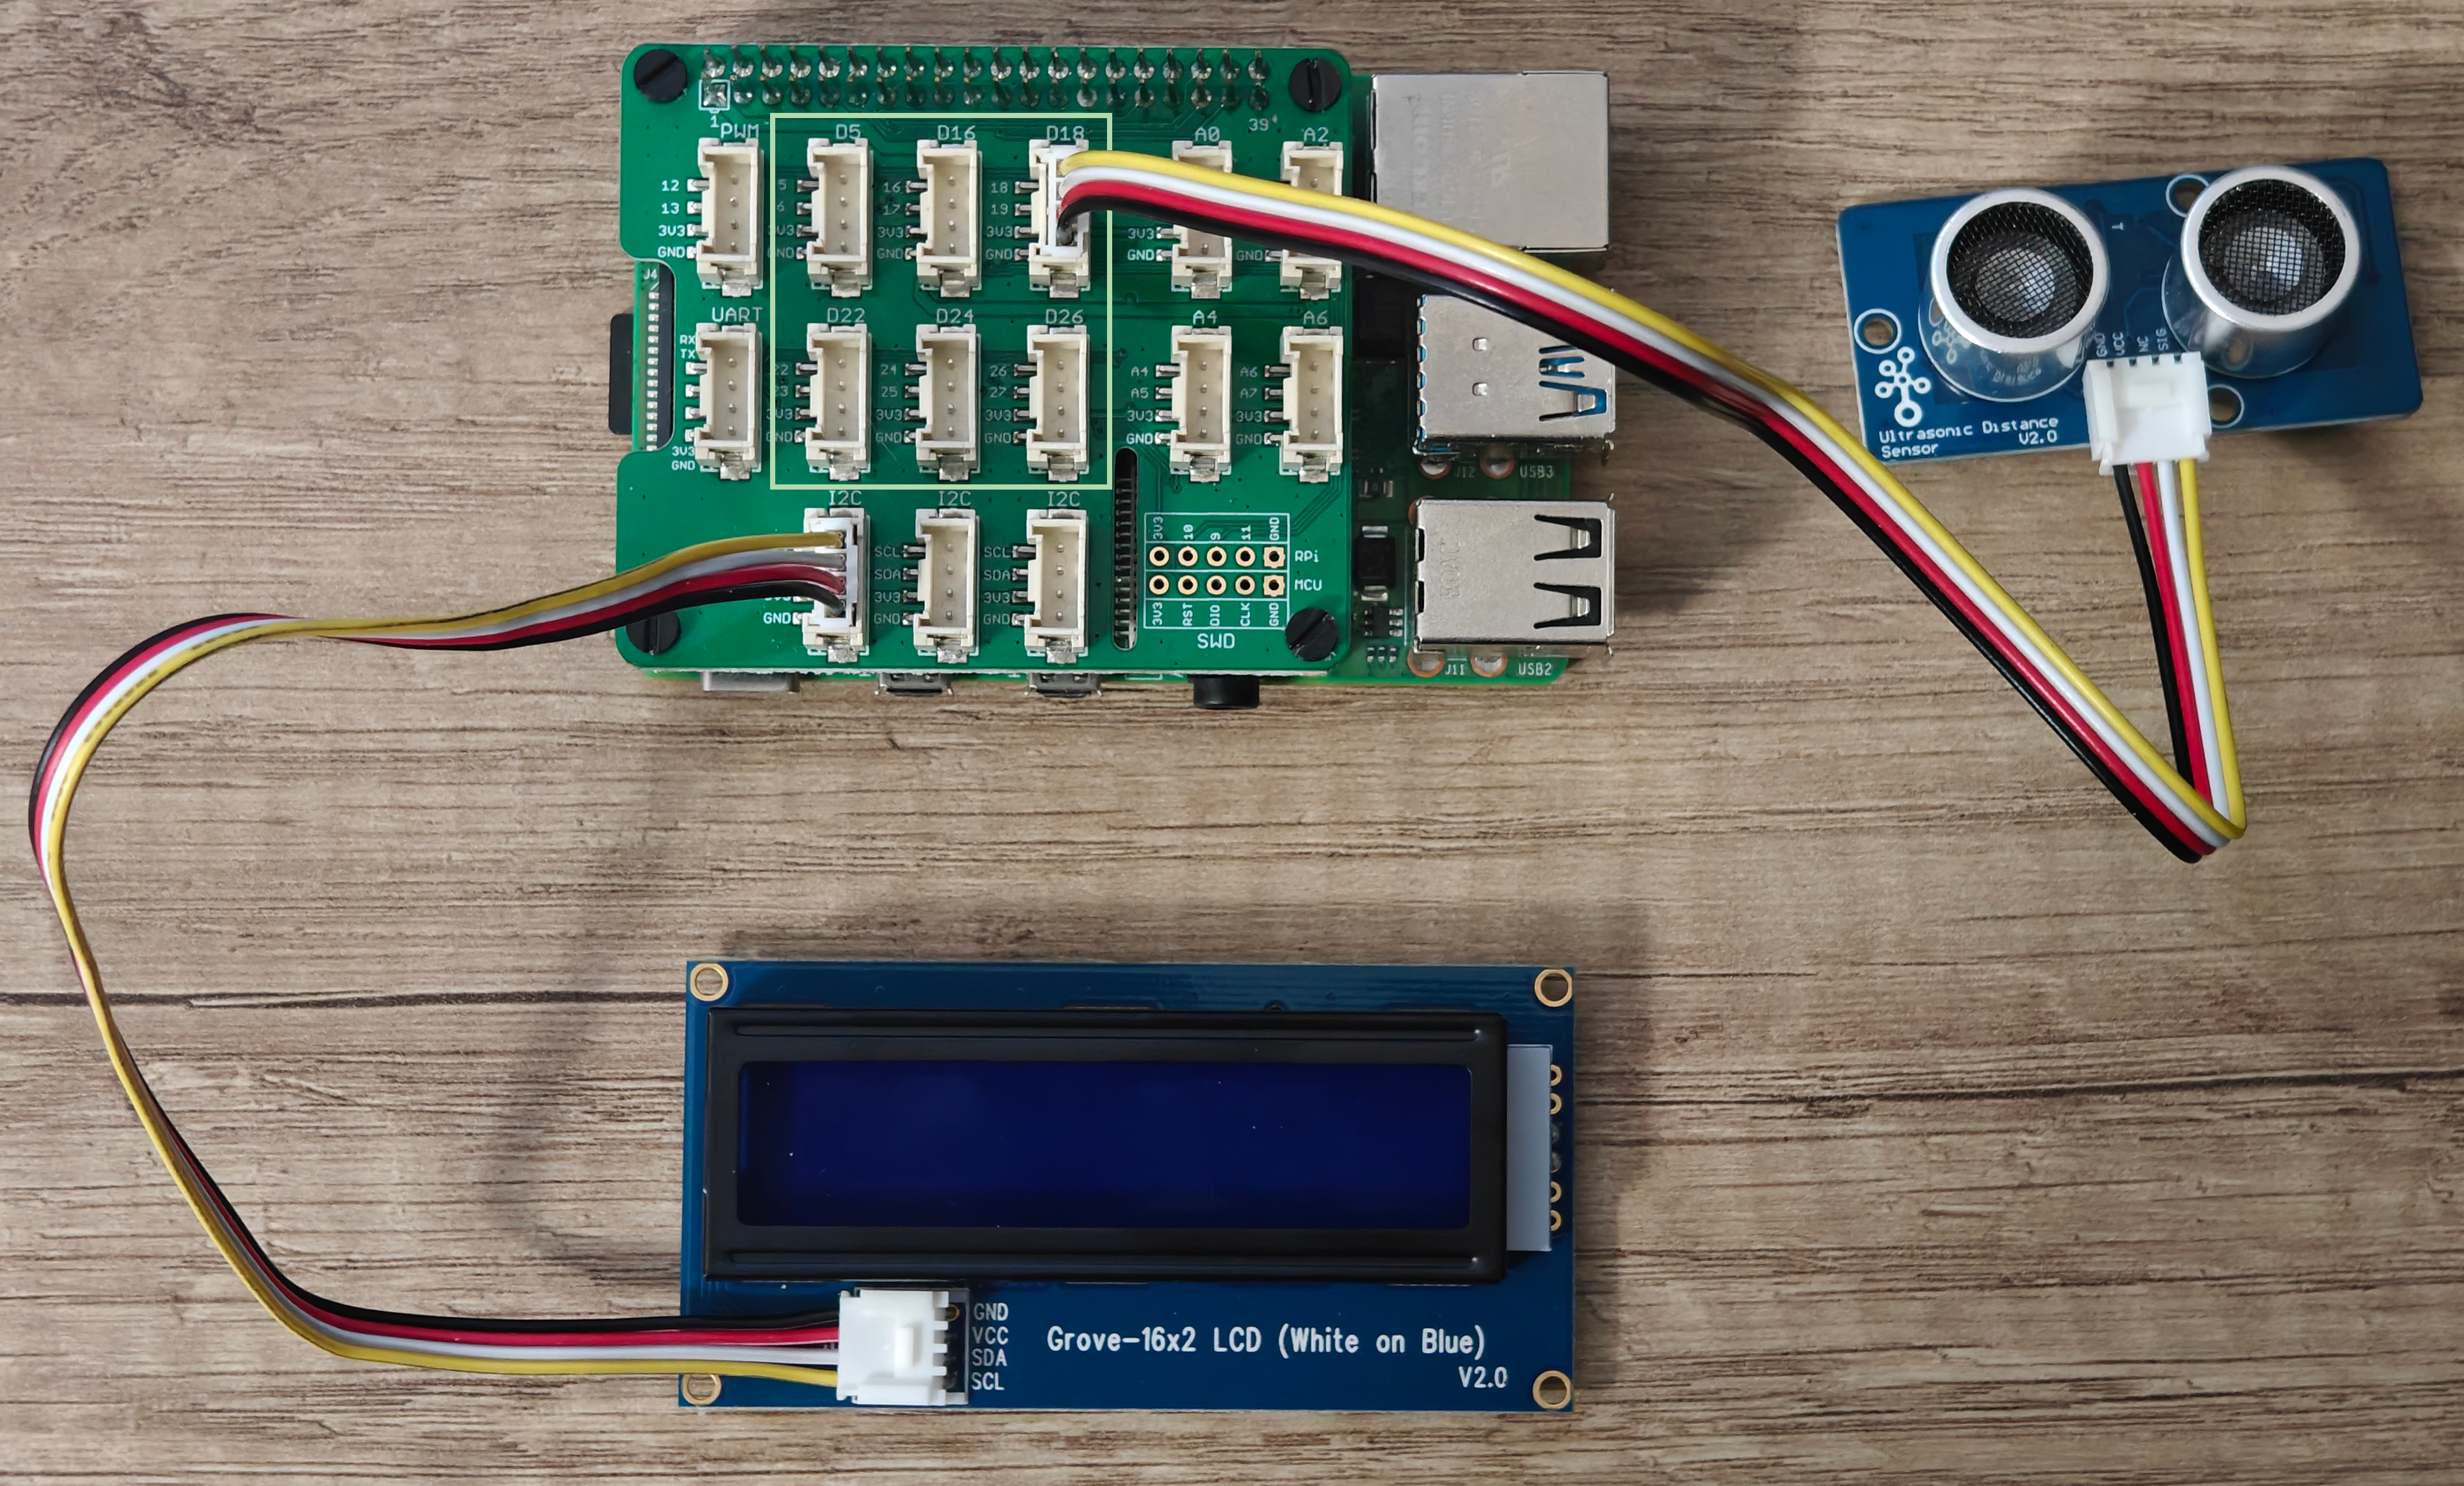
\includegraphics[width=0.7\linewidth]{media/grove_lcd_sonic}\\
  \caption{Montaż rozszerzenia -- moduł ultradźwiękowy}
  \label{fig:grovelcdsonic}
\end{figure}

\newpage
\setcounter{figure}{0}
\setcounter{chapter}{4}
{\chapnamefont \thechapter. Laboratorium III}

Laboratorium wykorzystuje \emph{Grove Base HAT} -- podłącz najpierw ten~moduł.

Czujnik ruchu wykorzystuje port \textbf{cyfrowy}.
Laboratorium zawiera zadanie odczytania podłączonego numeru portu -- wykorzystaj losowy z~portów cyfrowych
[\ref{fig:grovepir}].

\begin{figure}[H]
  \centering
  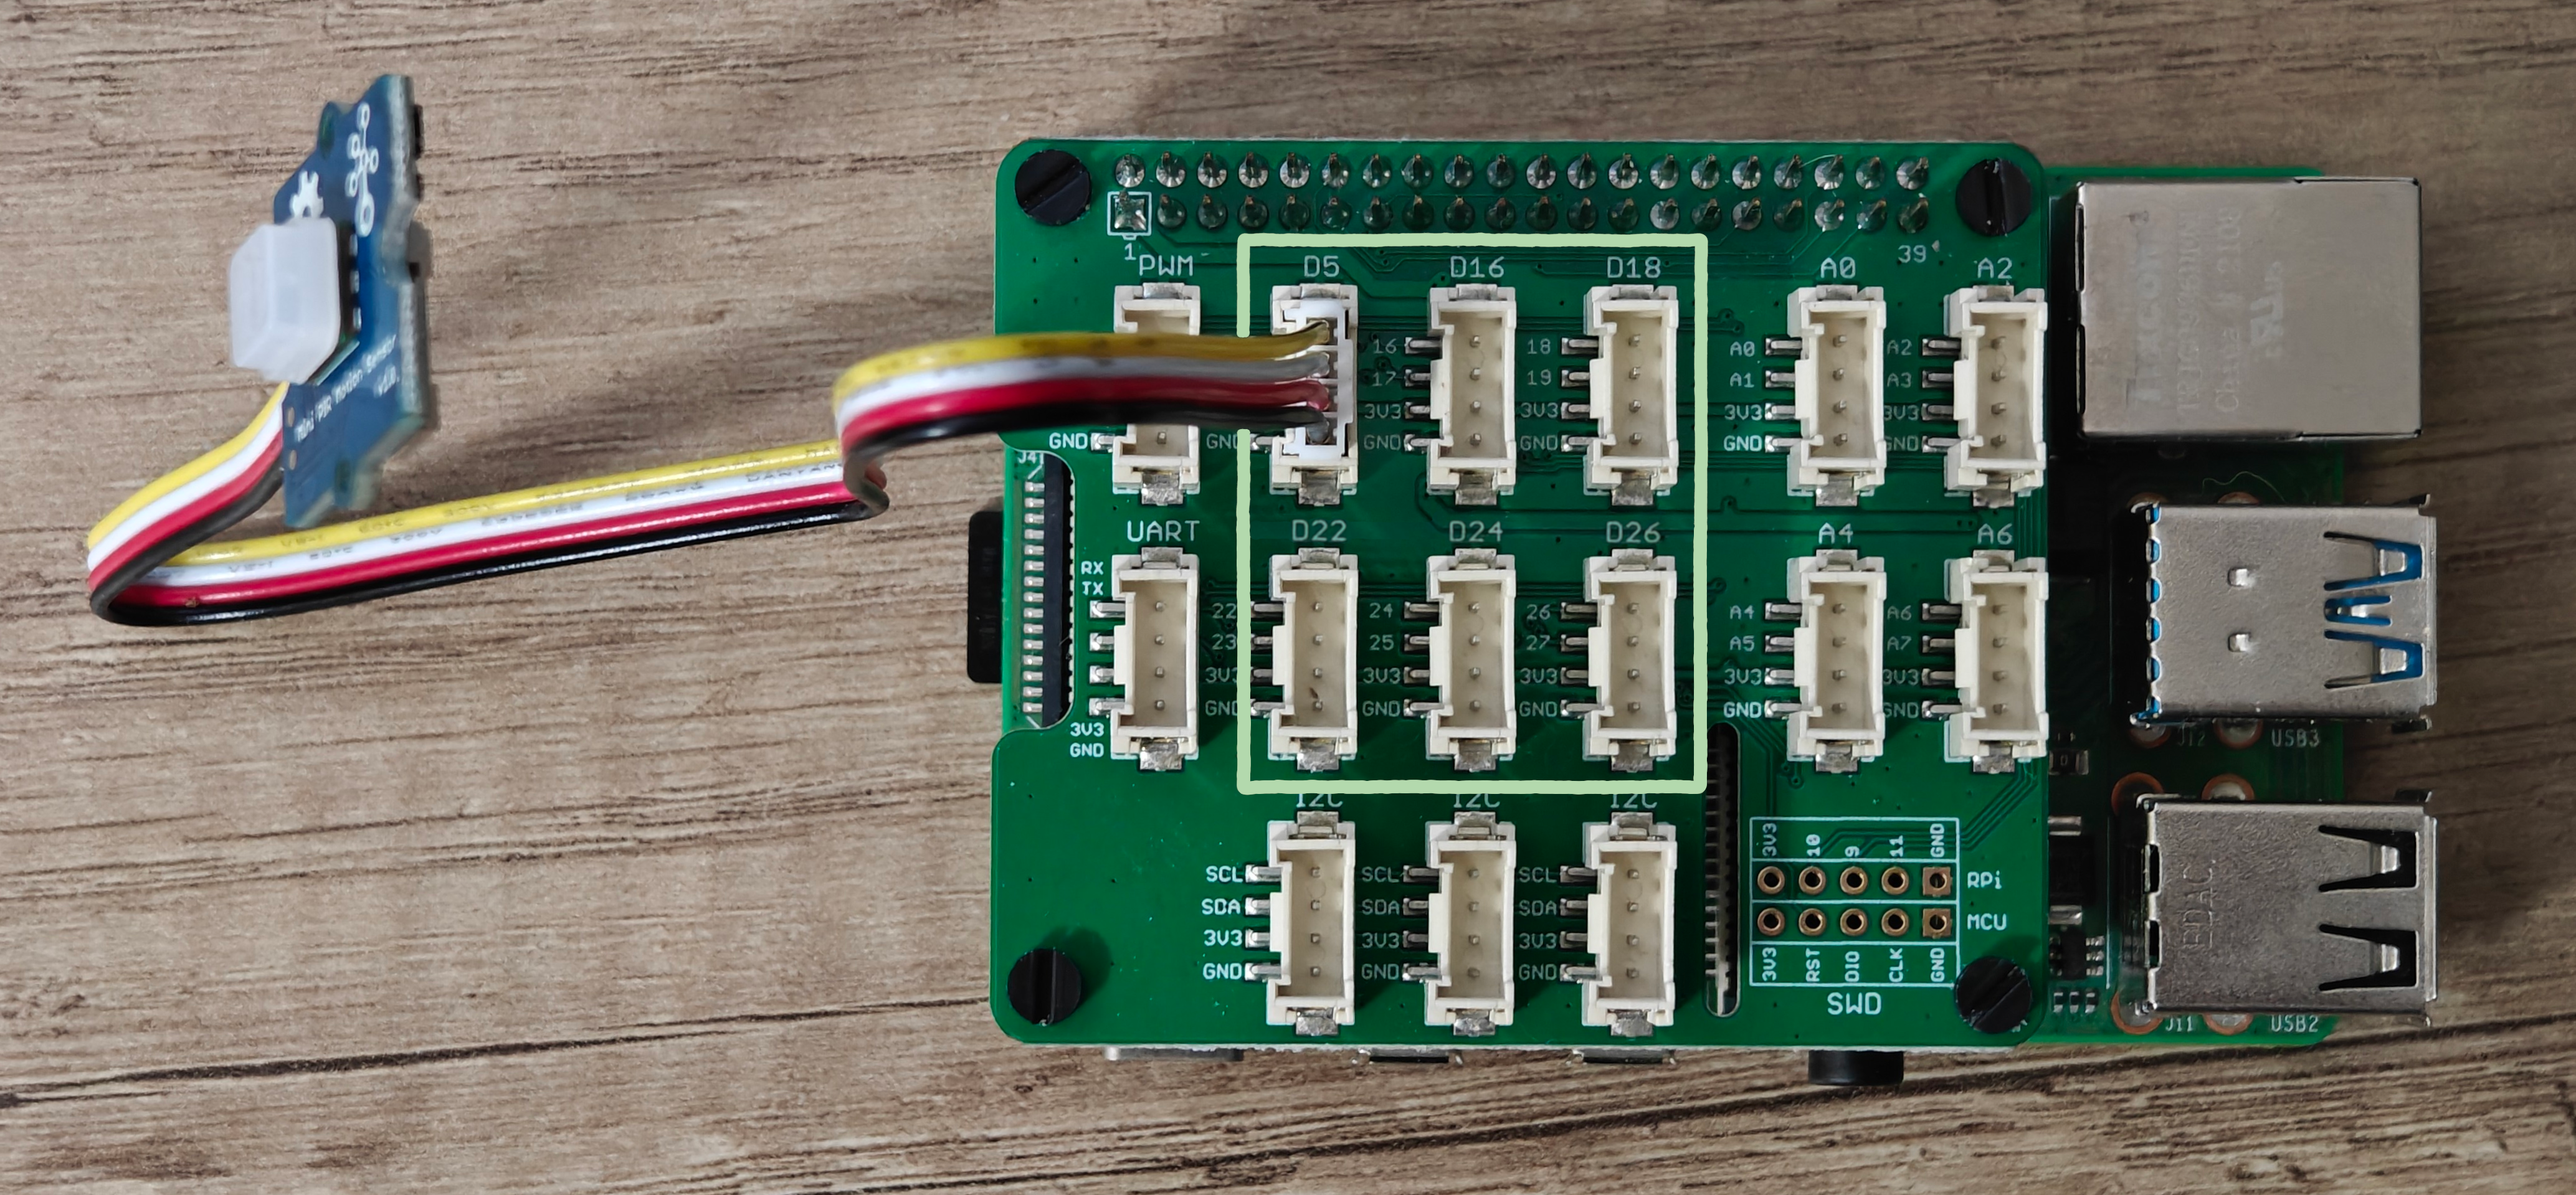
\includegraphics[width=0.55\linewidth]{media/grove_pir}\\
  \caption{Montaż rozszerzenia -- czujnik ruchu}
  \label{fig:grovepir}
\end{figure}

Przycisk LED wykorzystuje port \textbf{cyfrowy}.
Laboratorium zawiera zadanie odczytania podłączonego numeru portu -- wykorzystaj losowy z~portów cyfrowych
[\ref{fig:grovepirbtn}].

\begin{figure}[H]
  \centering
  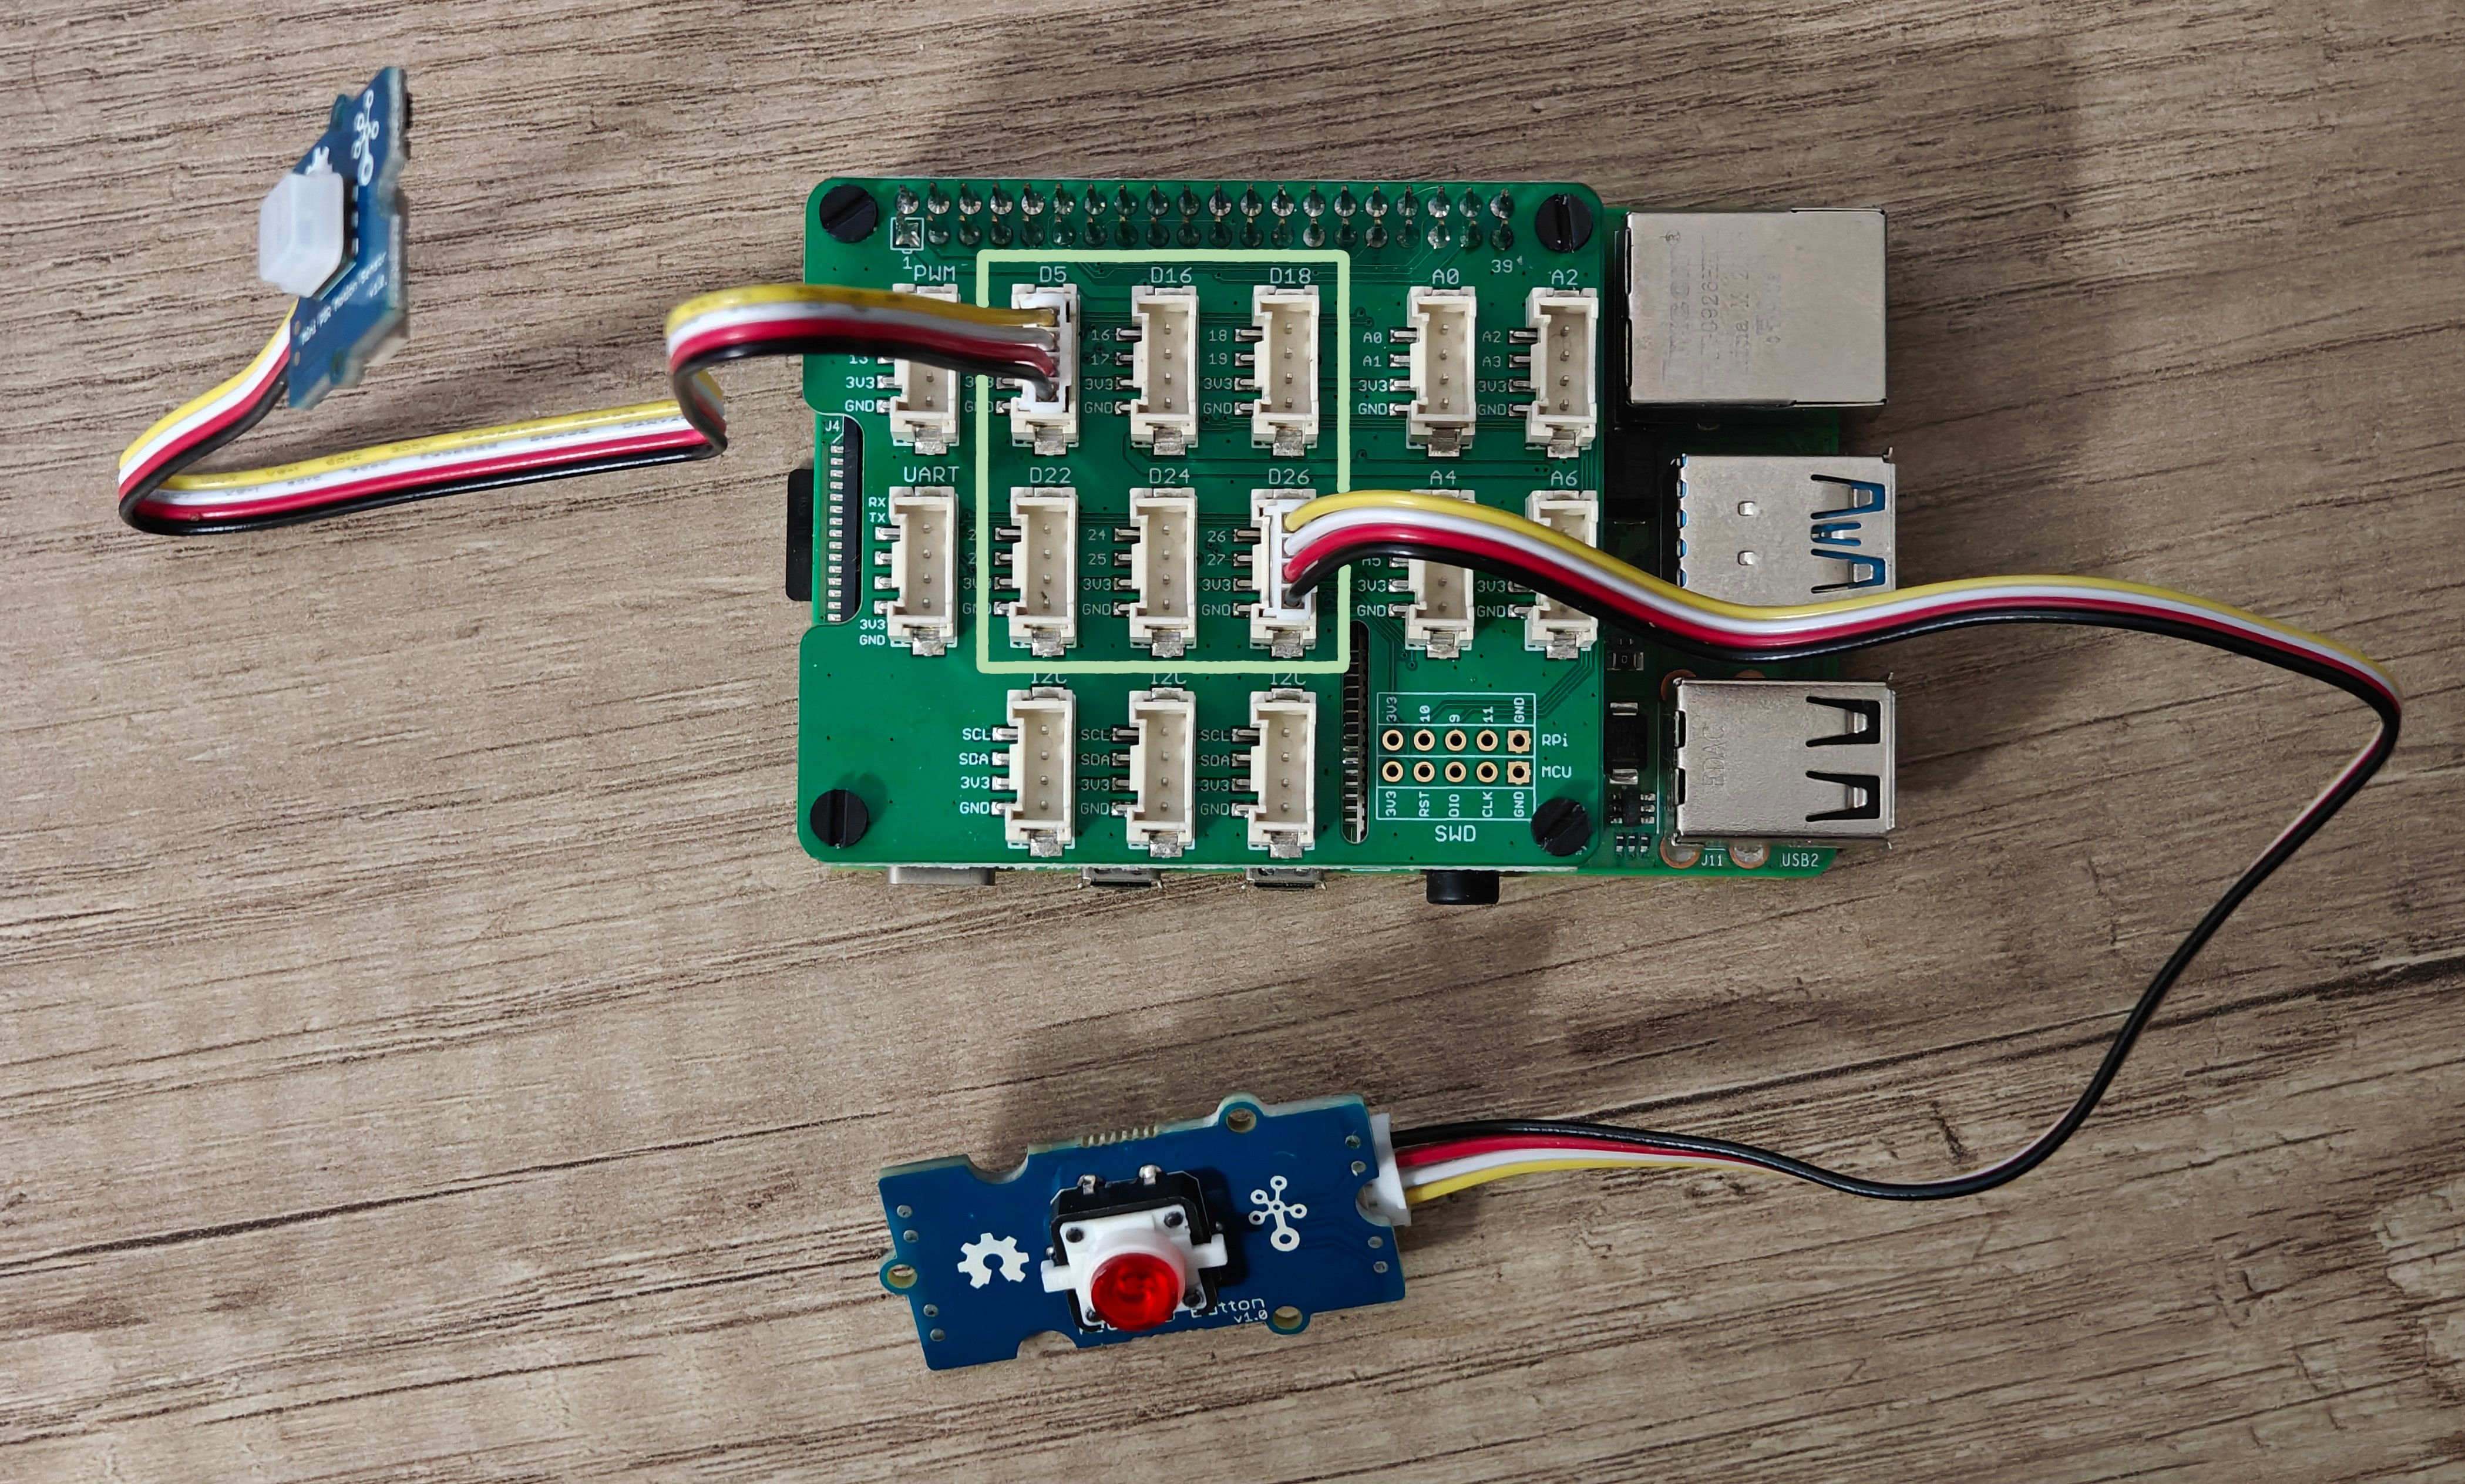
\includegraphics[width=0.7\linewidth]{media/grove_pir_btn}\\
  \caption{Montaż rozszerzenia -- przycisk LED}
  \label{fig:grovepirbtn}
\end{figure}

\newpage
\setcounter{figure}{0}
\setcounter{chapter}{5}
{\chapnamefont \thechapter. Laboratorium IV}

Moduł \emph{Enviro HAT} nie~ma widocznego na~poprzednio montowanych modułach wcięcia, ale~w~podobny sposób
można~wykorzystać cięcie odgradzające czujnik temperatury od~większej części modułu (kolor czerwony) wraz~z~otworami
wyprowadzającymi \emph{GPIO} (kolor żółty) [\ref{fig:envirohatunbuilt}].

\begin{figure}[H]
  \centering
  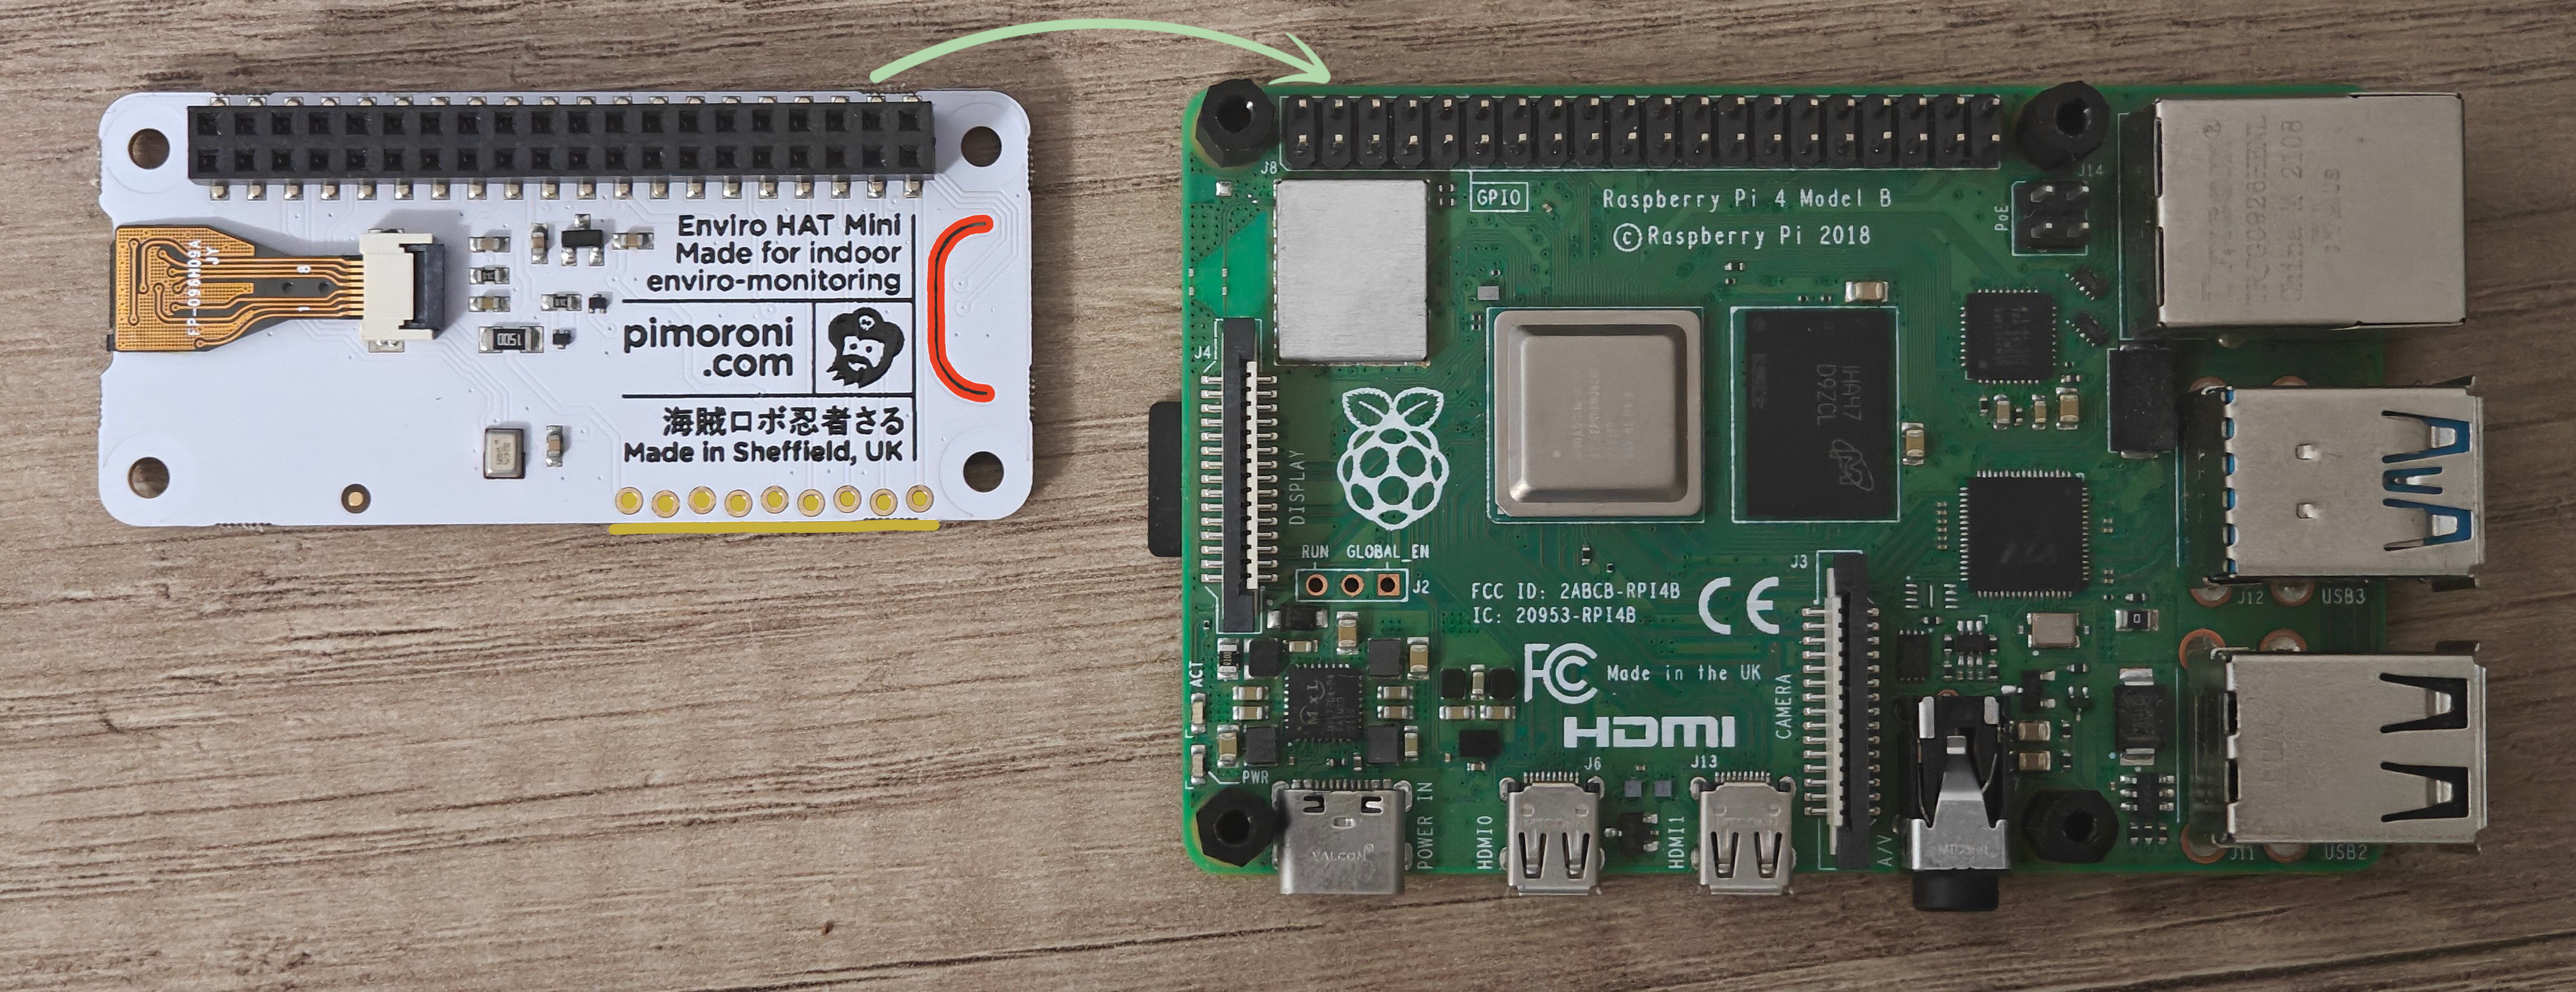
\includegraphics[width=\linewidth]{media/enviro_hat_unbuilt}\\
  \caption{Moduł \emph{Enviro HAT} obok płytki}
  \label{fig:envirohatunbuilt}
\end{figure}

Przymocowanie sprawi, że~to~cięcie będzie po~stronie lewej, a otwory nadal po~dolnej stronie [\ref{fig:envirohatbuilt}].

\begin{figure}[H]
  \centering
  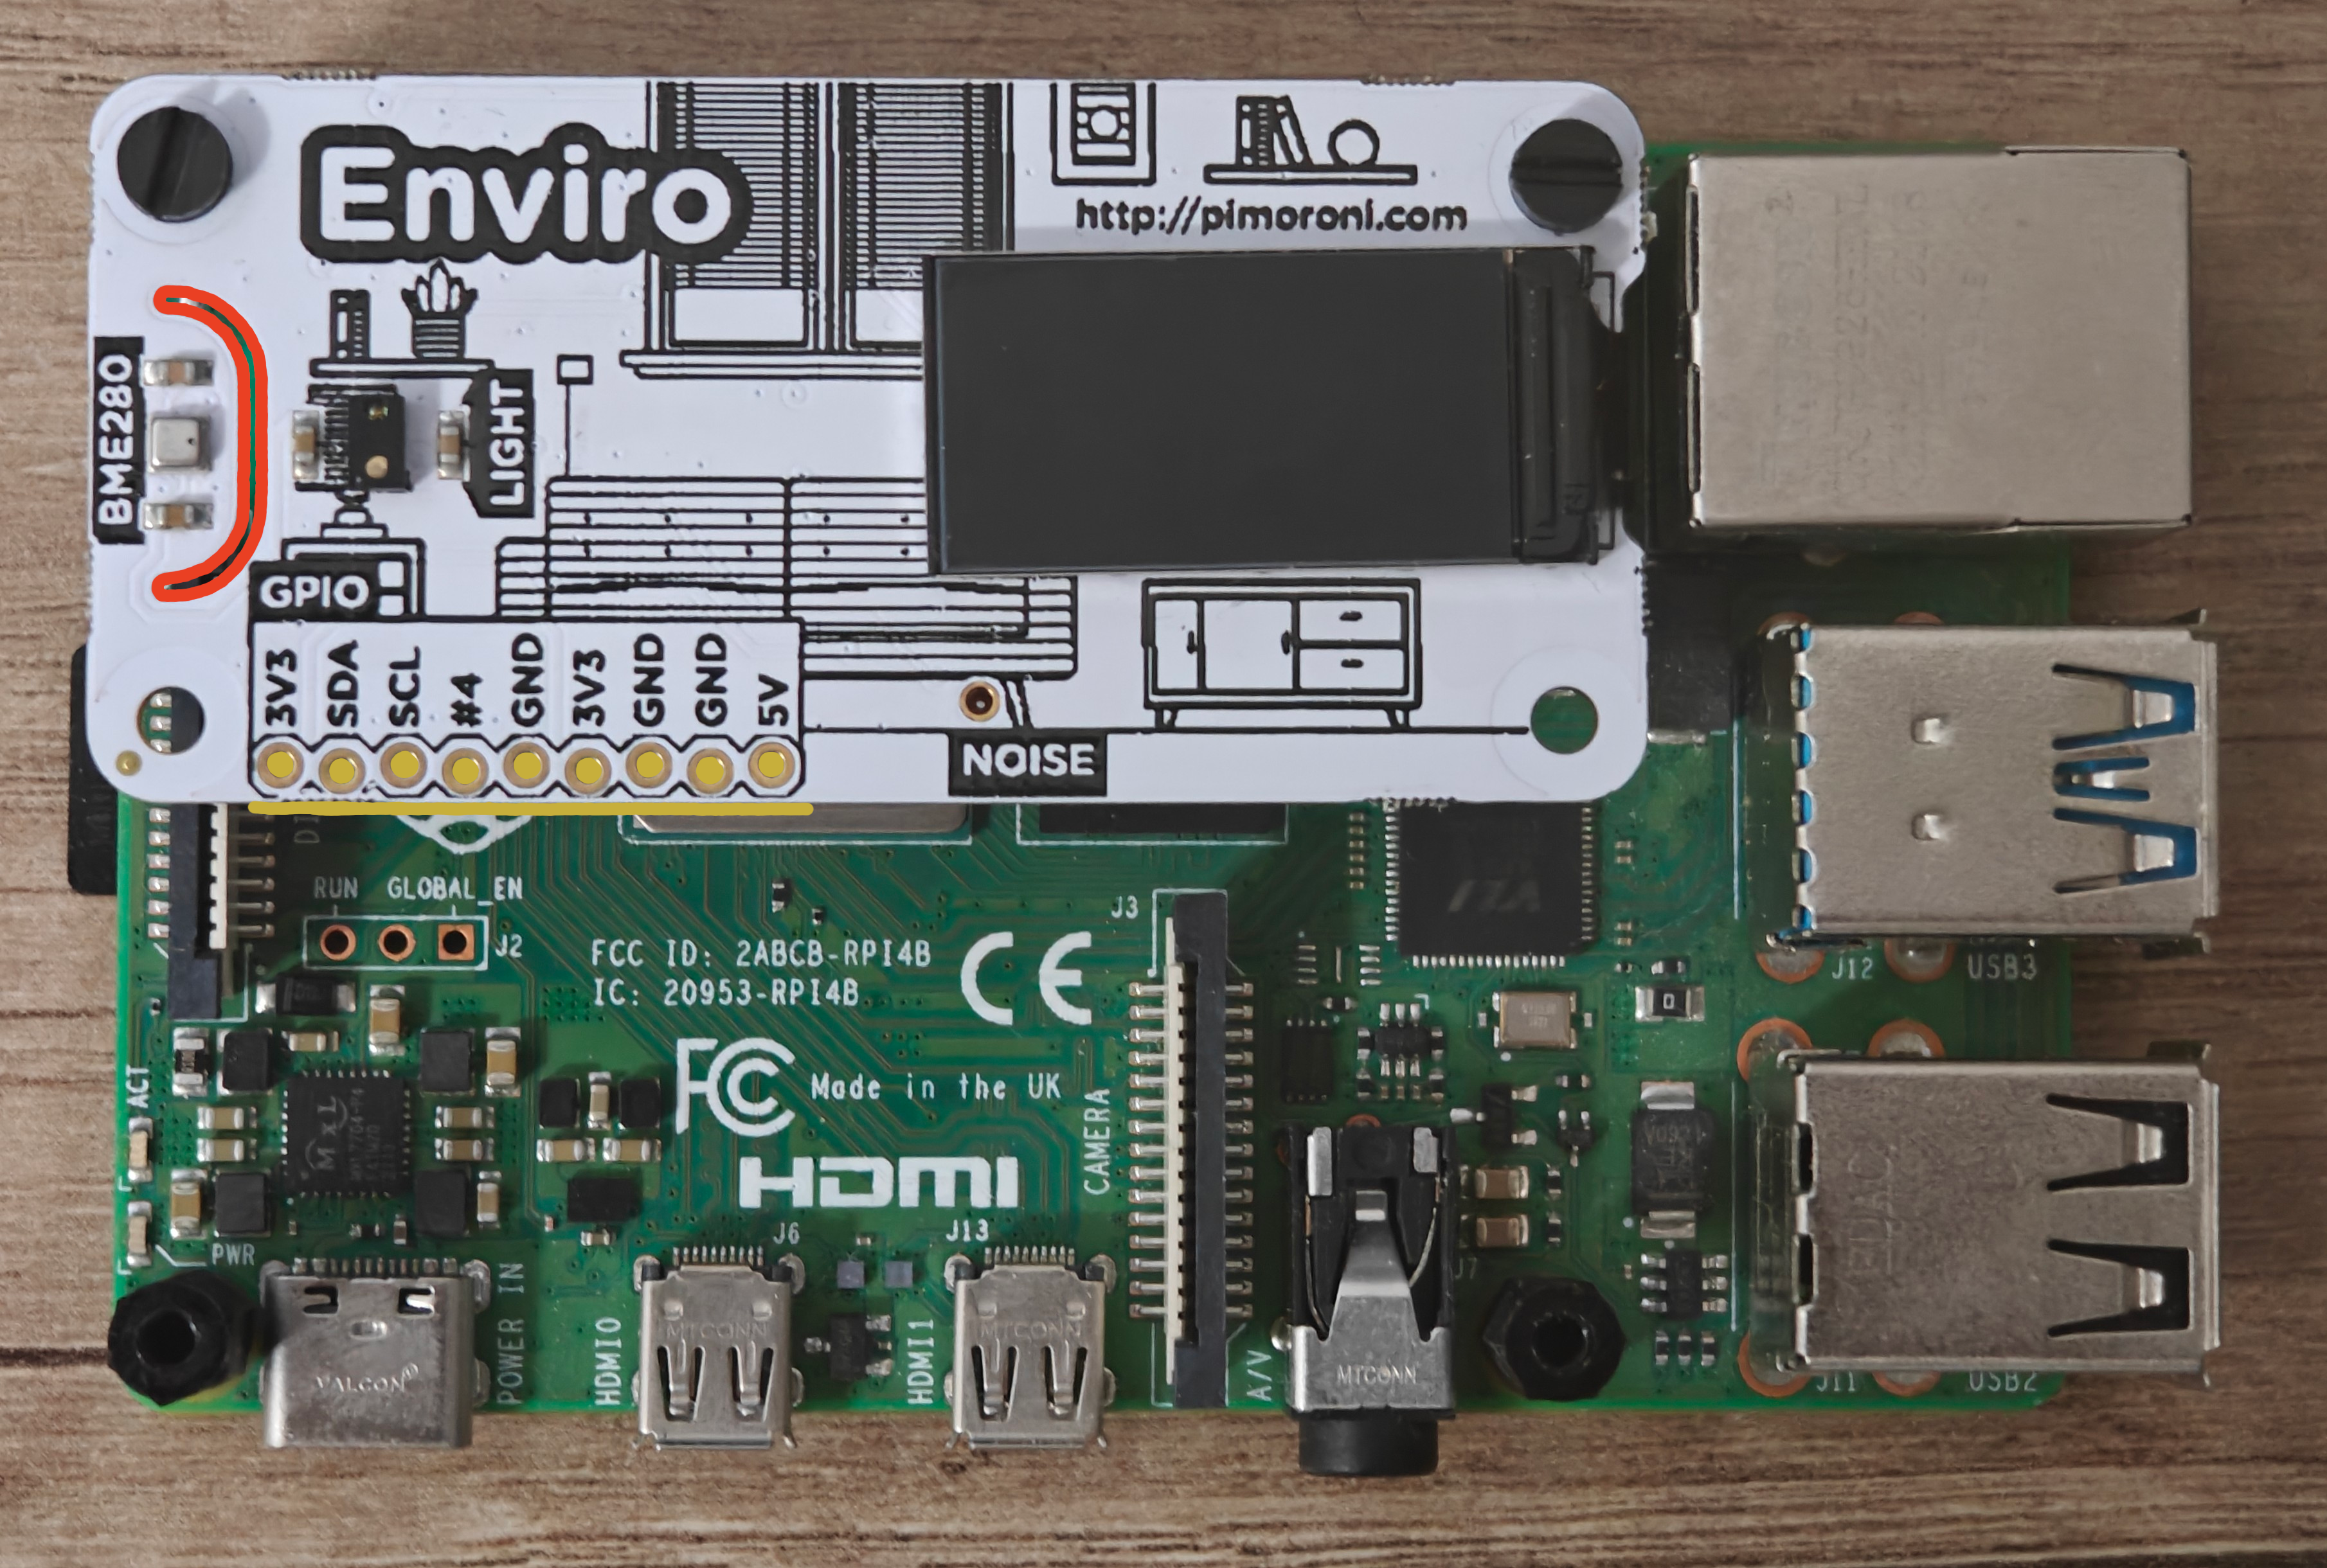
\includegraphics[width=0.6\linewidth]{media/enviro_hat_built}\\
  \caption{Przymocowany moduł \emph{Enviro HAT}}
  \label{fig:envirohatbuilt}
\end{figure}

\newpage
\setcounter{figure}{0}
\setcounter{chapter}{6}
{\chapnamefont \thechapter. Laboratorium V}

Moduł \emph{Traffic pHAT} również~różni~się od~poprzednich modułów, ale~w~podobny sposób do~pomocy w~orientacji
można~wykorzystać złącza elementu oznaczonego \emph{RN2} (kolor czerwony) i~dolny otwór montażowy (kolor żółty)
[\ref{fig:traffichatunbuilt}].

\begin{figure}[H]
  \centering
  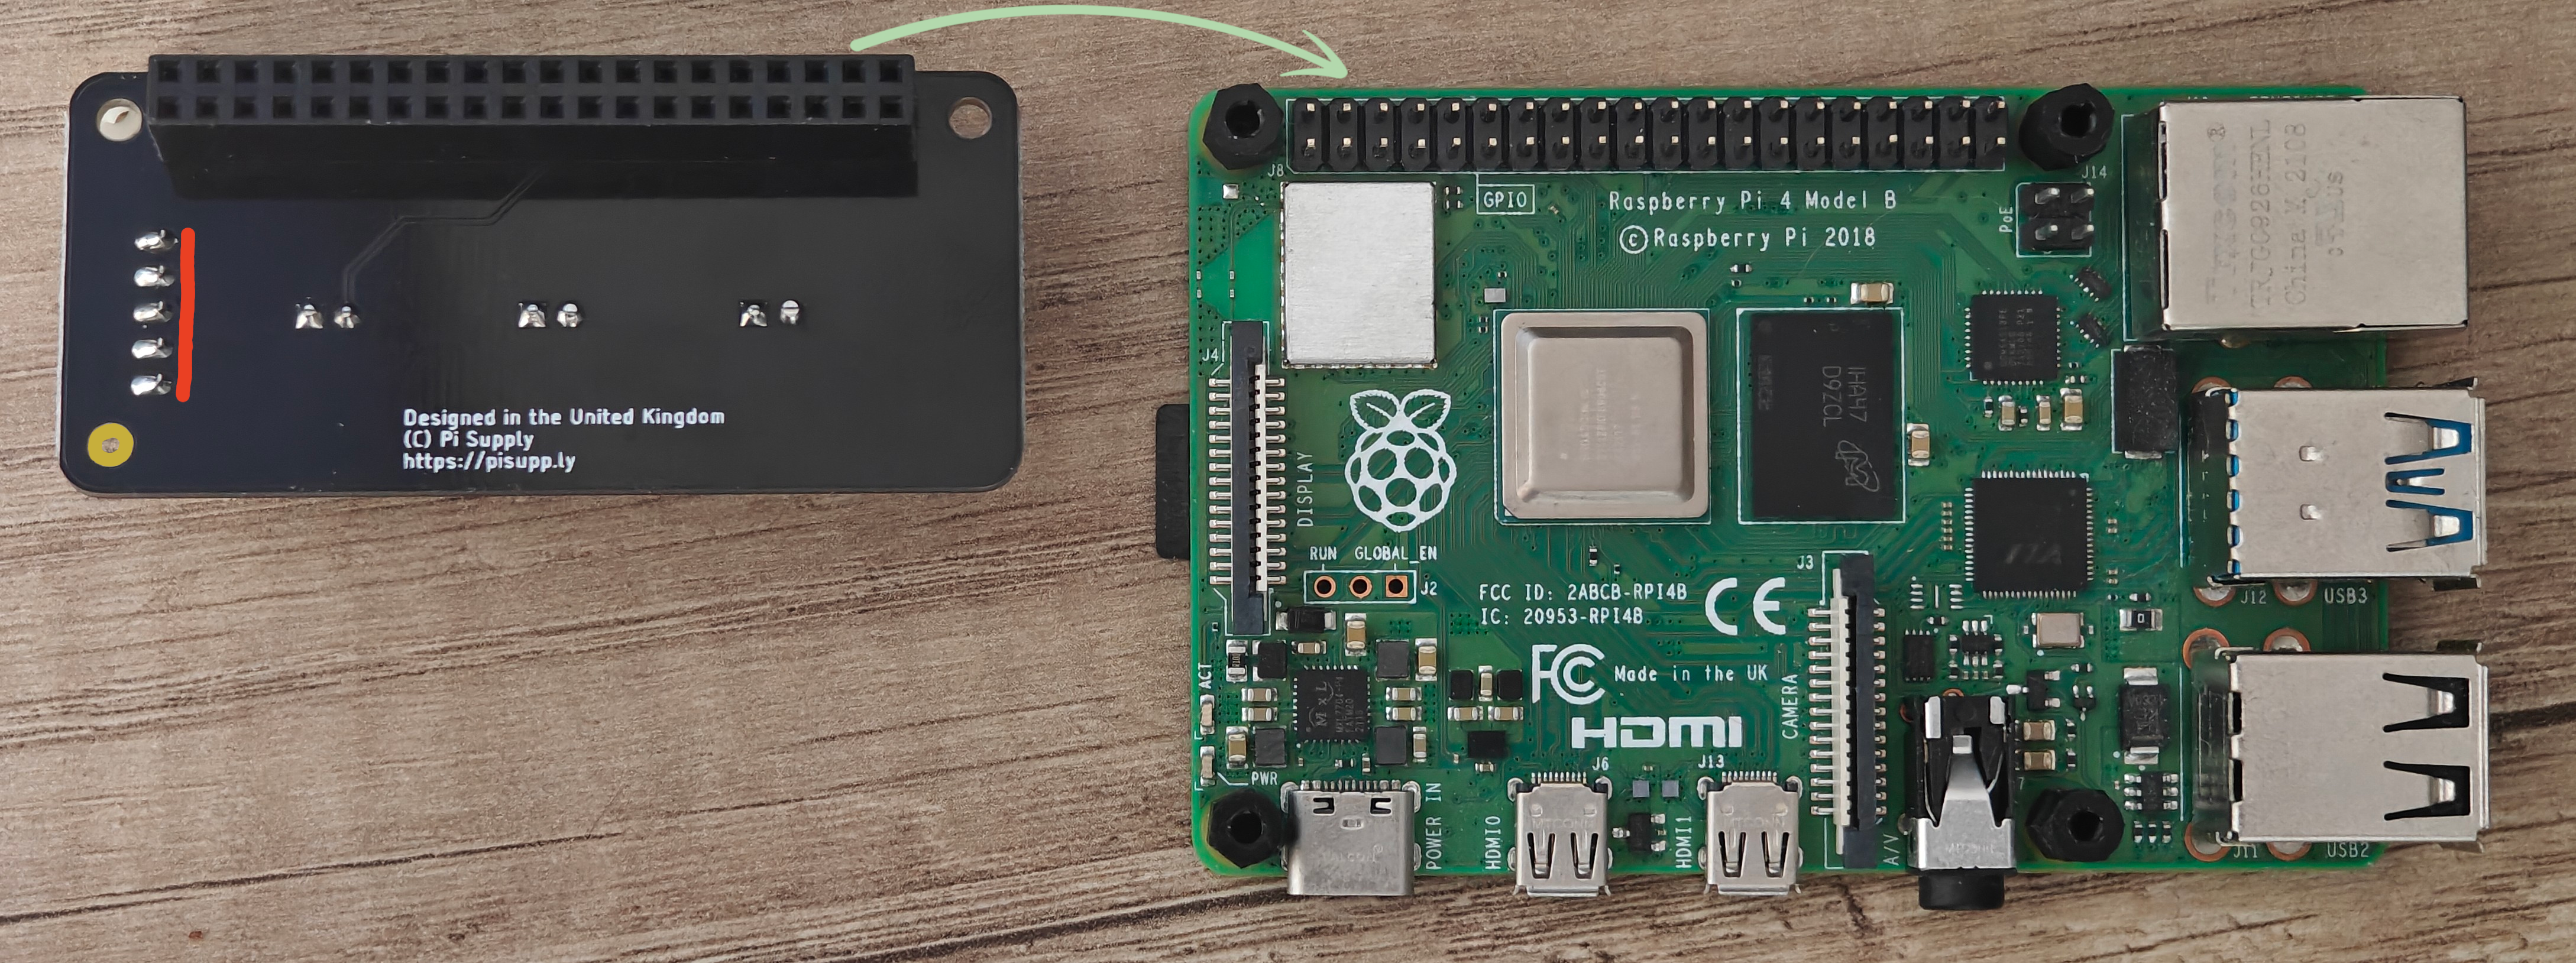
\includegraphics[width=\linewidth]{media/traffic_unbuilt}\\
  \caption{Moduł \emph{Traffic pHAT} obok płytki}
  \label{fig:traffichatunbuilt}
\end{figure}

Po~przymocowaniu modułu zaznaczone elementy będą~jak~w~poprzednich modułach odbiciem lustrzanym stanu początkowego
[\ref{fig:traffichatbuilt}].

\begin{figure}[H]
  \centering
  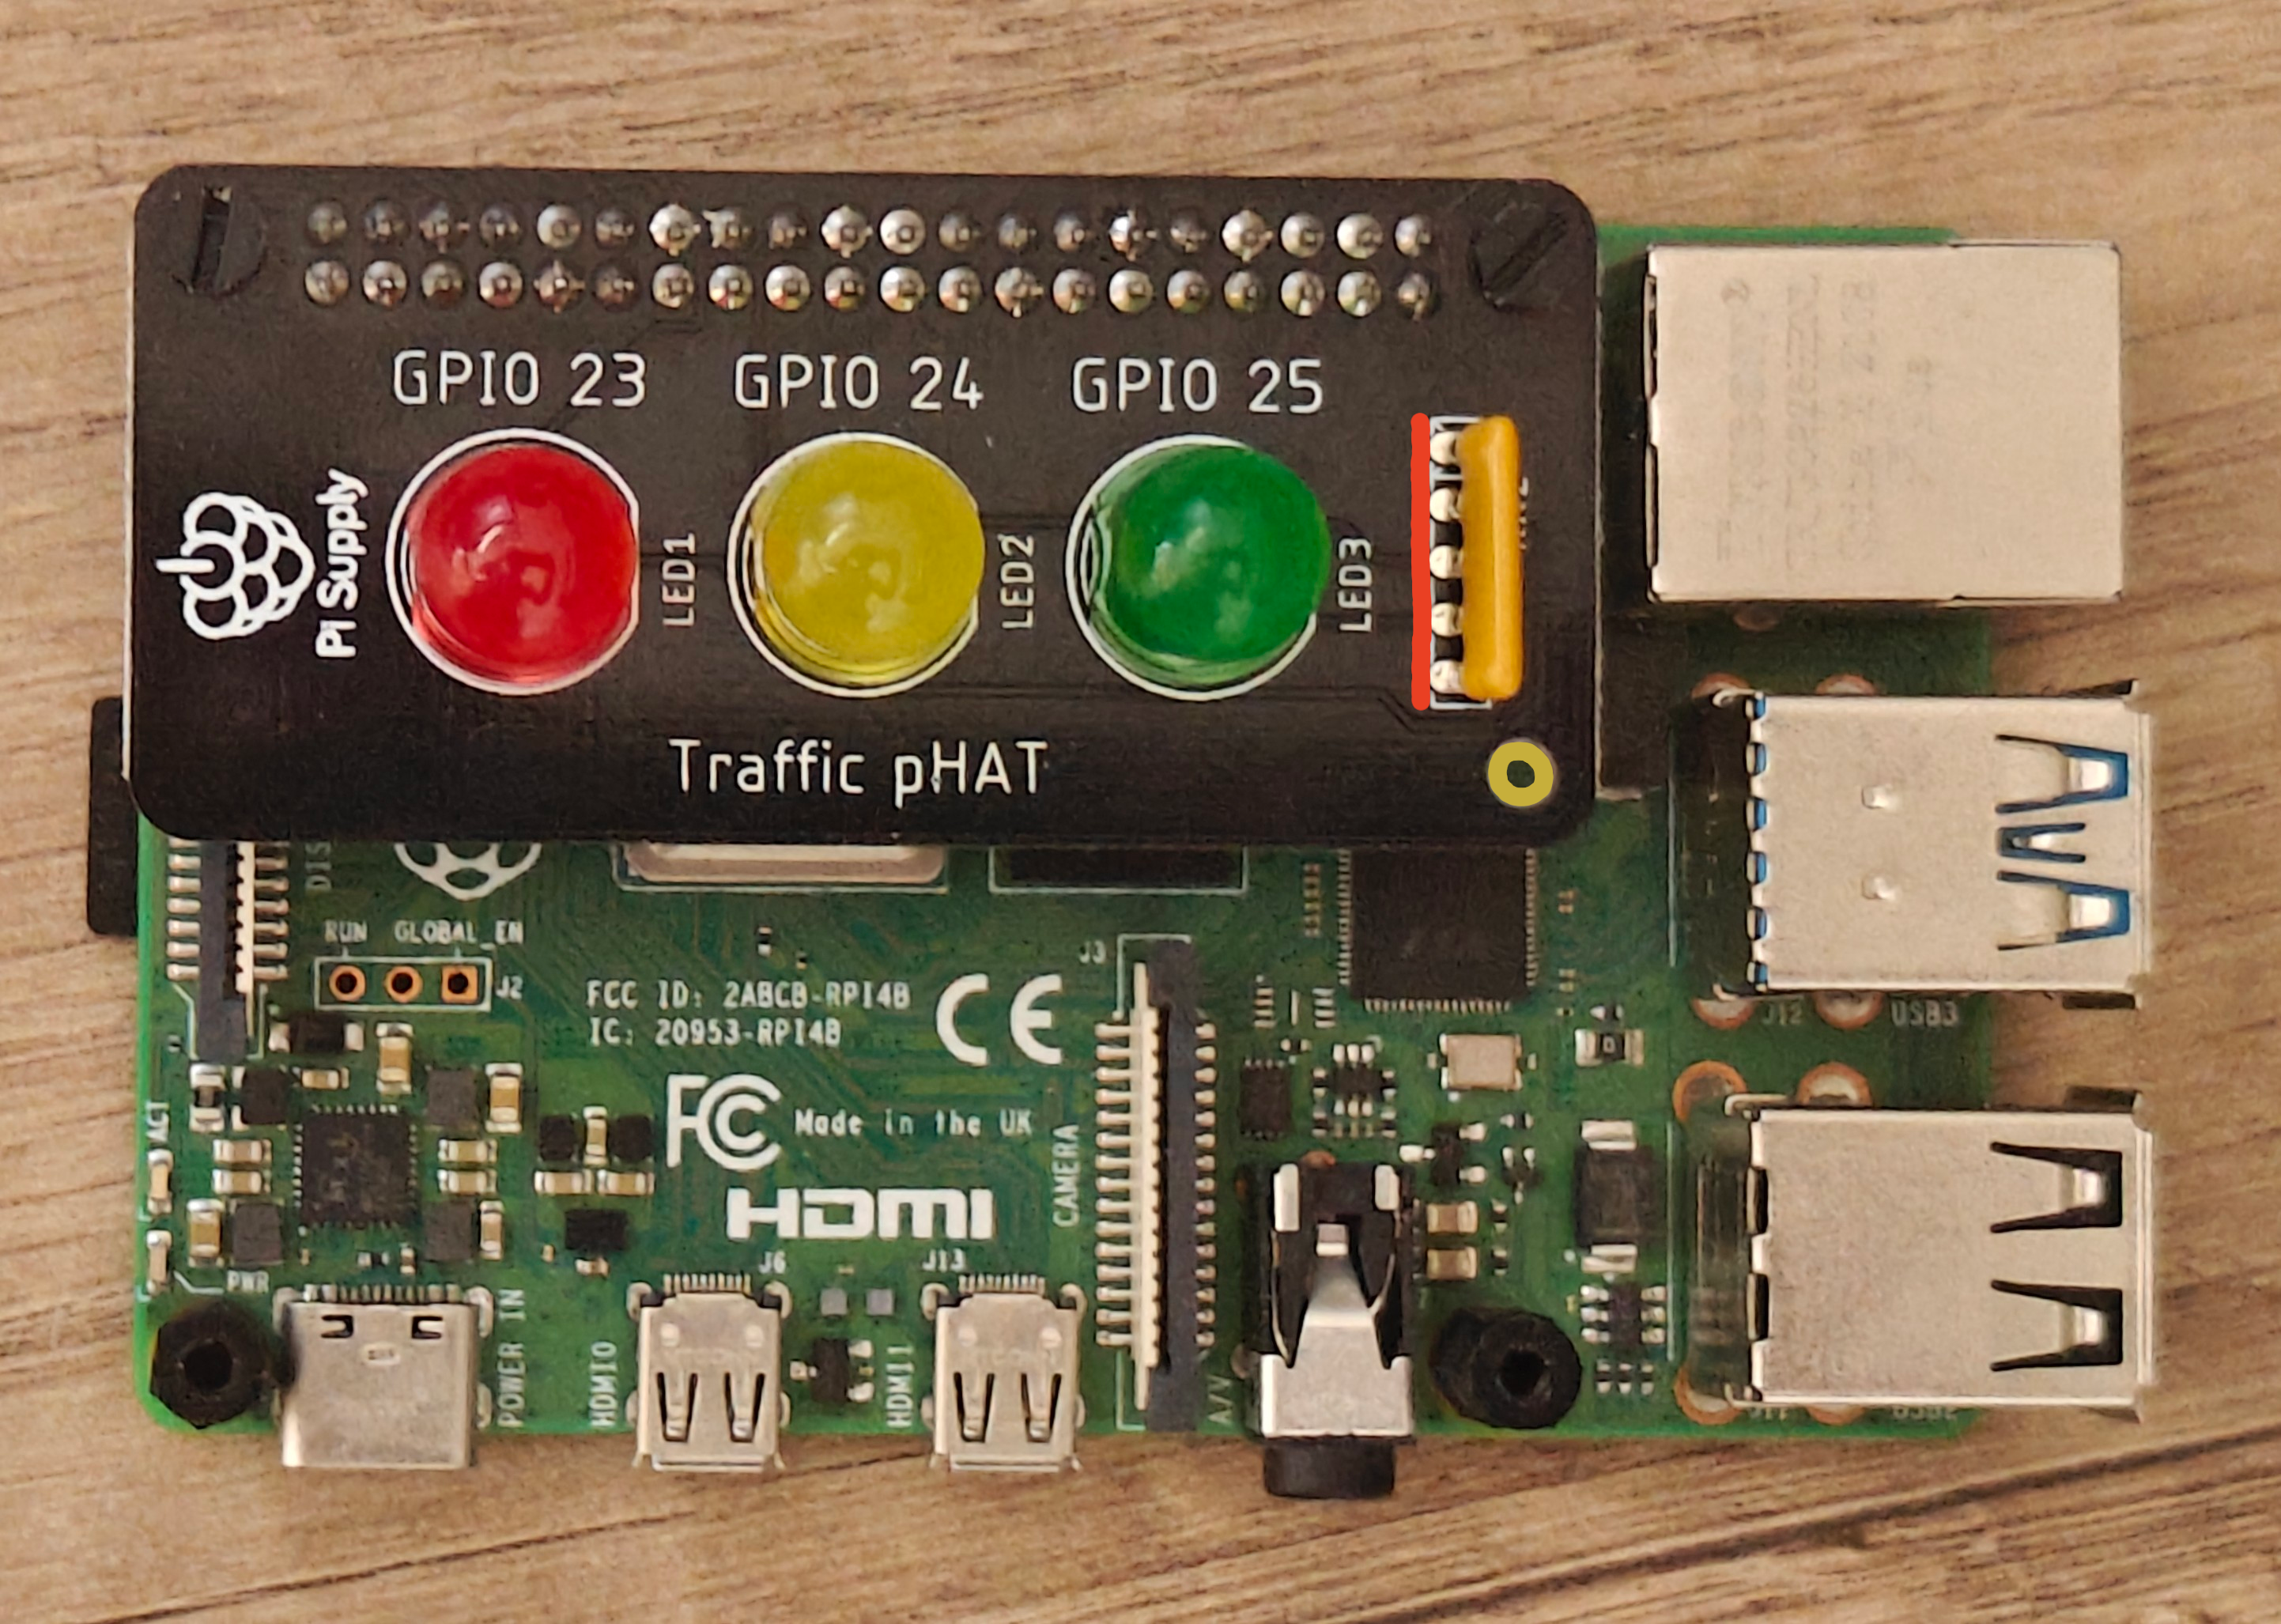
\includegraphics[width=0.6\linewidth]{media/traffic_built}\\
  \caption{Przymocowany moduł \emph{Traffic pHAT}}
  \label{fig:traffichatbuilt}
\end{figure}

\end{document}
